%%%%%%%%%%%%%%%%%%%%%%%%%%%%%%%%%%%%%%%%%
% Tufte-Style Book (Minimal Template)
% LaTeX Template
% Version 1.0 (5/1/13)
%
% This template has been downloaded from:
% http://www.LaTeXTemplates.com
%
% License:
% CC BY-NC-SA 3.0 (http://creativecommons.org/licenses/by-nc-sa/3.0/)
%
% IMPORTANT NOTE:
% In addition to running BibTeX to compile the reference list from the .bib
% file, you will need to run MakeIndex to compile the index at the end of the
% document.
%
%%%%%%%%%%%%%%%%%%%%%%%%%%%%%%%%%%%%%%%%%

%----------------------------------------------------------------------------------------
%	PACKAGES AND OTHER DOCUMENT CONFIGURATIONS
%----------------------------------------------------------------------------------------

\documentclass{tufte-book} % Use the tufte-book class which in turn uses the tufte-common class

\hypersetup{colorlinks} % Comment this line if you don't wish to have colored links

\usepackage{microtype} % Improves character and word spacing

\usepackage{lipsum} % Inserts dummy text

\usepackage{booktabs} % Better horizontal rules in tables

\usepackage{graphicx} % Needed to insert images into the document
\graphicspath{{graphics/}} % Sets the default location of pictures
\setkeys{Gin}{width=\linewidth,totalheight=\textheight,keepaspectratio} % Improves figure scaling

\usepackage{fancyvrb} % Allows customization of verbatim environments
\fvset{fontsize=\normalsize} % The font size of all verbatim text can be changed here

\newcommand{\hangp}[1]{\makebox[0pt][r]{(}#1\makebox[0pt][l]{)}} % New command to create parentheses around text in tables which take up no horizontal space - this improves column spacing
\newcommand{\hangstar}{\makebox[0pt][l]{*}} % New command to create asterisks in tables which take up no horizontal space - this improves column spacing

\usepackage{xspace} % Used for printing a trailing space better than using a tilde (~) using the \xspace command

\usepackage{amssymb} % Used for more unusual symbols are not defined in base LaTeX(NFSS)

\usepackage{amsmath} % Used for many rare mathematical symbols.

\newcommand{\monthyear}{\ifcase\month\or January\or February\or March\or April\or May\or June\or July\or August\or September\or October\or November\or December\fi\space\number\year} % A command to print the current month and year

\newcommand{\openepigraph}[2]{ % This block sets up a command for printing an epigraph with 2 arguments - the quote and the author
\begin{fullwidth}
\sffamily\large
\begin{doublespace}
\noindent\allcaps{#1}\\ % The quote
\noindent\allcaps{#2} % The author
\end{doublespace}
\end{fullwidth}
}

\setcounter{secnumdepth}{0} % Count until chapter for titles and references
\setcounter{tocdepth}{1} % Show until section in contents

\newcommand{\blankpage}{\newpage\hbox{}\thispagestyle{empty}\newpage} % Command to insert a blank page

\usepackage{units} % Used for printing standard units

\newcommand{\hlred}[1]{\textcolor{Maroon}{#1}} % Print text in maroon
\newcommand{\hangleft}[1]{\makebox[0pt][r]{#1}} % Used for printing commands in the index, moves the slash left so the command name aligns with the rest of the text in the index 
\newcommand{\hairsp}{\hspace{1pt}} % Command to print a very short space
\newcommand{\ie}{\textit{i.\hairsp{}e.}\xspace} % Command to print i.e.
\newcommand{\eg}{\textit{e.\hairsp{}g.}\xspace} % Command to print e.g.
\newcommand{\na}{\quad--} % Used in tables for N/A cells

\newcommand{\doccmddef}[2][]{\hlred{\texttt{#2}}\label{cmd:#2}\ifthenelse{\isempty{#1}} % Command to define a command in red and add it to the index
{ % If no package is specified, add the command to the index
\index{#2 command@\protect\hangleft{}\texttt{#2}}% Command name
}
{ % If a package is also specified as a second argument, add the command and package to the index
\index{#2 command@\protect\hangleft{}\texttt{#2} (\texttt{#1} package)}% Command name
\index{#1 package@\texttt{#1} package}\index{packages!#1@\texttt{#1}}% Package name
}}

% A bunch of new commands to print commands, arguments, environments, classes, etc within the text using the correct formatting
\newcommand{\mono}[1]{\texttt{#1}}
\newcommand{\tabincell}[2]{\begin{tabular}{@{}#1@{}}#2\end{tabular}} 

\usepackage{makeidx} % Used to generate the index
\makeindex % Generate the index which is printed at the end of the document

% This block contains a number of shortcuts used throughout the book

%----------------------------------------------------------------------------------------
%	BOOK META-INFORMATION
%----------------------------------------------------------------------------------------

\title{Statistical Methods for Astroparticle Physics} % Title of the book

\author[G. Benato]{G. Benato} % Author

\publisher{Gran Sasso Science Institute} % Publisher

%----------------------------------------------------------------------------------------

\begin{document}

\frontmatter

%----------------------------------------------------------------------------------------

\maketitle % Print the title page

%----------------------------------------------------------------------------------------
%	COPYRIGHT PAGE
%----------------------------------------------------------------------------------------

\newpage
\begin{fullwidth}
~\vfill
\thispagestyle{empty}
\setlength{\parindent}{0pt}
\setlength{\parskip}{\baselineskip}
Copyright \copyright\ \the\year\ \thanklessauthor

\par\smallcaps{By \thanklesspublisher}

\par\smallcaps{\url{http://www.bookwebsite.com}}

\par License information.\index{license}

\par\textit{First printing, \monthyear}
\end{fullwidth}

%----------------------------------------------------------------------------------------

\tableofcontents % Print the table of contents

%----------------------------------------------------------------------------------------

\listoffigures % Print a list of figures

%----------------------------------------------------------------------------------------

\listoftables % Print a list of tables

%----------------------------------------------------------------------------------------

\mainmatter


%----------------------------------------------------------------------------------------
%	INTRODUCTION
%----------------------------------------------------------------------------------------

\cleardoublepage
\chapter{Introduction} % The asterisk leaves out this chapter from the table of contents
\label{ch:intro}

\section{Language conventions}\index{language conventions}

\newthought{Language conventions} are sometimes different between physicists and statisticians.

\begin{table} % Add the following just after the closing bracket on this line to specify a position for the table on the page: [h], [t], [b] or [p] - these mean: here, top, bottom and on a separate page, respectively
	\centering % Centers the table on the page, comment out to left-justify
	\begin{tabular}{c c} % The final bracket specifies the number of columns in the table along with left and right borders which are specified using vertical bars (|); each column can be left, right or center-justified using l, r or c. To specify a precise width, use p{width}, e.g. p{5cm}
		\toprule % Top horizontal line
		Physicist says & Statistician says\\ % Column names row
		\midrule % In-table horizontal line
		determine & estimate\\ % Content row 1
		estimate & guess\\ % Content row 2
		\bottomrule % Bottom horizontal line
	\end{tabular}
	\caption{Language example 1} % Table caption, can be commented out if no caption is required
	\label{tab:LangEx1} % A label for referencing this table elsewhere, references are used in text as \ref{label}
\end{table}

\begin{table}
	\centering
	\begin{tabular}{c c}
		\toprule
		Demographic language & Physics language\\
		\midrule
		Sample & Data (set)\\
		Draw a sample & Observe, measure\\
		Sample of size $N$ & $N$ observations \\
		Population & Observable space\\
		\bottomrule
	\end{tabular}
	\caption{Language example 2}
	\label{tab:LangEx2}
\end{table}

\begin{itemize}[$\to$]
	\item Think about a census, or an election poll. 
		\marginnote{We will specify: “Parent mean = population mean = mean of the underlying distribution” 
		
		or: “sample mean”}
	\item We need to distinguish between the properties of the sample and these of the underlying population.
\end{itemize}

Avoid \mono{misleading terms}\index{language conventions!misleading terms}:

\begin{itemize}
	\item error $\to$ variance, confidence interval, interval estimate, credible interval
	\item propagation of error $\to$ change of variable
\end{itemize}

\section{Two philosophies}

\begin{itemize}[$\to$]
	\item \newthought{Bayesian} approach\index{Bayesian approach} measures the “degree of belief”\index{degree of belief} that a statement is true.
	\item \newthought{Frequentist} approach\index{frequentist approach} measures the relative frequency of something happening.
\end{itemize}

\begin{table}
	\centering
	\begin{tabular}{c c c}
		\toprule
		& Bayesian & Frequentist\\
		\midrule
		Statement depends on observer & $\times$ & \\
		Applier to repeatable cases & $\times$ & $\times$\\
		Applier to future unknown facts & $\times$ & \\
		Applier to past unknown facts & $\times$ & \\
		Applier to possible outcome of an experiment & $\times$ & \\
		Applier to the true value of a parameter & $\times$ & \\
		\tabincell{c}{Allows goodness-of-fit \\ (single hypothesis testing)} & & $\times$\\
		Allows decision theory & $\times$ & \\
		\bottomrule
	\end{tabular}
	\caption{Two philosophies}
	\label{tab:2philosophies}
\end{table}

\section{Notation} \index{language conventions!notation}

\begin{itemize}[$\to$]
	\item \mono{Greek letters}: parameters of the theory: $\theta$, $\mu$, $\sigma$, $\cdots$
	\item \mono{Roman letters}: random variable corresponding to physical observables: $x$, $E$, $\cdots$
	\item \mono{Capitalized}: $P$, probability distribution\index{probability distribution}; $F$, cumulative distribution\index{cumulative distribution}
	\item \mono{Lowercase}: $p$ or $f$, probability density function\index{probability density function}
	\item \mono{Bar}: average value: $\bar{x}$, $\bar{E}$, $\cdots$
	\item \mono{Hat}: estimate of parameter (often mode\index{mode} of the parameter): $\hat{\theta}$, $\hat{\mu}$, $\hat{\sigma}$, $\cdots$
\end{itemize}



%----------------------------------------------------------------------------------------
%	PROBABILITY THEORY
%----------------------------------------------------------------------------------------

\chapter{Probability theory}
\label{ch:prob}


%------------------------------------------------

\section{History}

\begin{fullwidth}
\lipsum[5]
\end{fullwidth}

\subsection{Subsection 1}

\lipsum[6-7]

\subsection{Subsection 2}

\lipsum[7-8]



%------------------------------------------------

\section{Definition of probability}\index{probability}
\label{sec:def_of_prob}

\subsection{Mathematical probability}\index{mathematical probability}

\lipsum[6-7]

\subsection{Frequentist probability}\index{frequentist probability}

\lipsum[7-8]

\subsection{Bayesian probability}\index{Bayesian probability}
\label{subsec:bayesian_prob}

\paragraph{Degree of belief}\index{degree of belief}

Amount $F(x)$ that we are willing to bet that $x$ will occur.

Knowing that if we win, we will get a fixed amount $k$.
\marginnote{This is called \mono{coherent bet}\index{coherent bet}.}

\begin{equation}
	\to P(x) = \frac{F(x)}{k}
\end{equation}

\begin{equation}
	\to \left\{
	\begin{array}{rcl}
		P(x) = 0 & & {\textrm{if we are sure } x \textrm{ will not happen,}}\\
		P(x) = 1 & & {\textrm{if we are sure } x \textrm{ will happen,}}\\
		0 < P(x) < 1 & & {\textrm{otherwise.}}
	\end{array} \right.
\end{equation}

\begin{equation}\label{eq:norm_cond}
	\sum_{i} P(n_{i}) = 1
\end{equation}

\begin{itemize}
	\item It is a property of the system to be observed, as well as the observer.
	\item It depends on the knowledge of the observer, and will change if the knowledge of the observer improves.
	\item Can be applied to non-repeatable phenomenon.
		\marginnote{Italy winning the next world cup; 
		
		me getting bold;
		
		or the aliens to have colonized the Earth in prehistoric times.}
	\item Can be applied to the true value of a physics theory!
\end{itemize}

\subsection{Applicability of frequentist and Bayesian probability}\index{probability!applicability}
\label{subsec:app_prob}

\newthought{Based on these definitions}, we can immediately make a decision on which type of probability to use depending on the situation, i.e. depending on the question that we want to address. This is particularly important is we consider the fact that the physical parameter of a theory are fixed by Nature, but unknown to us.

For example, we can ask the following types of question:

\begin{itemize}[$\to$] 
	\item Based on the result of a measurement, what is the true value of a parameter of the theory?
	\item Based on the result of a measurement, what is the interval that contains the true (unknown) value of a given parameter with a given amount of probability?
	\item Is my parameterization of the measured data good enough? Or does it indicate the presence of some “new physics”?
	\item Supposing I want to compare two alternative models based on some experimental data, which of the models describes better the data?
	\item Based on the results of previous experiments, what is the expected outcome of a future experiment measuring the same quantity, or a quantity connected to it?
\end{itemize}



%------------------------------------------------

\section{Properties of estimators}\index{estimator!property}
\label{sec:point_estimation_prop_of_estimator}

\subsection{Consistency}\index{consistency}
\label{subsec:prop_of_estimator_consistency}

\subsection{Efficiency}\index{efficiency}
\label{subsec:prop_of_estimator_efficiency} Minimum variance and Cramér–Rao inequality

Neglecting the bias, the smaller the variance of the estimatorm, the more certain we are that the estimate is near the true value of the parameter. 

One can prove that the variance $V(\hat{\theta})$ of any consistent estimation is subject to a lower bound given by:
\begin{align}
    V(\hat{\theta}) \geq \underset{V_{CR}(\hat{\theta})}{\underbrace{\dfrac{\Big ( 1 + \dfrac{\partial b(\hat{\theta})}{\partial \theta} \Big )}{E \Big [ \Big ( \dfrac{\partial \ln{\mathcal{L}(\vec{x}|\theta)}}{\partial \theta} \Big )^2 \Big]}}} \genfrac{}{}{3pt}{}{\leftarrow {\text{Bias of estimator}}}{\leftarrow \text{Fisher information}} 
\end{align}

We define the efficiency of the estimator as: $\epsilon(\hat{\theta}) = \dfrac{V_{CR}(\hat\theta)}{V(\hat{\theta})}$. 
Any consistent estimator $\hat{\theta}$ has an efficiency whihc is at most equal to $1$.

\section{Properites of maximum likelihood}
\label{sec:point_estimation_prop_of_max_likelihood}

We need to distinguish between 

\to asymptotic properties \to hold for sufficiently large $n$





%------------------------------------------------

\section{Random variables and probability distributions}\index{random variable}\index{probability distribution}
\label{sec:rand_var}

\newthought{A random event} is an event that has more than one possible outcome, to which a probability may be associated.

The outcome of a random event is not known, only the probabilities of the possible outcomes are known.

We can associate a random variable $x$ to a random event $\mathbf{X}$.

The possible numerical values $x_{1}, x_{2}, \cdots$ corresponding to the possible outcomes are the probabilities $P(x_{1}), P(x_{2}), \cdots$, which forms a “probability distribution”\index{probability distribution}, obeying to the normalization condition (\ref{eq:norm_cond}).

\marginnote{ $ \sum_{i} P(n_{i}) = 1$ (\ref{eq:norm_cond})}

\begin{itemize}[$\to$]
	\item A set of $N$ observations of the random variable $x$ can be considered as a single observation of a vector $\vec{x} := (x_{1}, \cdots, x_{n})$.
	\item This is the definition of a histogram.
		\marginnote{What if a random variable covers a continuous interval?}
\end{itemize}

\subsection{Probability density function	}\index{probability density function}
\label{subsec:pdf}

Consider a sample space $\Omega \subset \mathbb{R}^{n}$.

A random extraction (experiment) will lead to an outcome (measurement) corresponding to one point $\vec{x} \in \Omega$.

We can associate a “probability density” $f(\vec{x})$ to any point $\vec{x} \in \Omega$, with $f(\vec{x}) \geq 0$.

The probability of an event $A$ is: 

\begin{equation}\label{eq:prob_event}
	P(A) = \int_{A} {f(\vec{x})} \,\mathrm{d}\vec{x}
\end{equation}

$f(\vec{x})$ is the differential probability, \ie the infinitesimal probability $\mathrm{d}P$ corresponding to the infinitesimal hyper-volume $\mathrm{d}\vec{x}$.

\begin{equation}\label{eq:differential_prob}
	f(\vec{x}) = \frac{\mathrm{d}P(\vec{x})}{\mathrm{d}\vec{x}}
\end{equation}

$f(\vec{x})$ obeys the normalization condition:

\begin{equation}\label{eq:differential_norm_cond}
	\int_{\Omega} {f(\vec{x})} \,\mathrm{d}\vec{x} = 1
\end{equation}

If $x$ is a 1-dim discrete variable:

\begin{equation}\label{eq:discrete_differential_prob}
	f(x) = \sum_{i = 1}^{n}{P_{i} \delta(x - x_{i})}
\end{equation}

In fact:

\begin{equation}
	\int_{-\infty}^\infty f(x) \,\mathrm{d}x = \sum_{i = 1}^{n}{P_{i} \int_{-\infty}^\infty \delta(x - x_{i}) \,\mathrm{d}x} = \sum_{i} P_{i} = 1
\end{equation}

If a variable is continuous, but we measure it with a discretized device, we can instead do:

\marginnote{This is the case of a measurement done with a MCA.

This is the case of a measurement of a particle track with a pixelated detector with pixel size $\delta x$.}

\begin{equation}
	P_{i} = \int_{x_{i}}^{x_{i} + \delta x} f(x) \,\mathrm{d}x
\end{equation}

\subsection{Cumulative distribution}\index{cumulative distribution}
\label{subsec:cdf}

\marginnote[6pt]{Monotonous increasing function from 0 to 1.}

It is defined as (\ref{eq:cumulative_distr}):

\begin{equation}\label{eq:cumulative_distr}
	F(x) = \int_{-\infty}^{x} f(y) \,\mathrm{d}y
\end{equation}

\begin{equation}
	F(\tilde{x}) = P(x \leq \tilde{x}) \,\forall \tilde{x}
\end{equation}

An example plot is (Figure~\ref{fig:CDF_PDF_Gaussian}):

\begin{figure}
	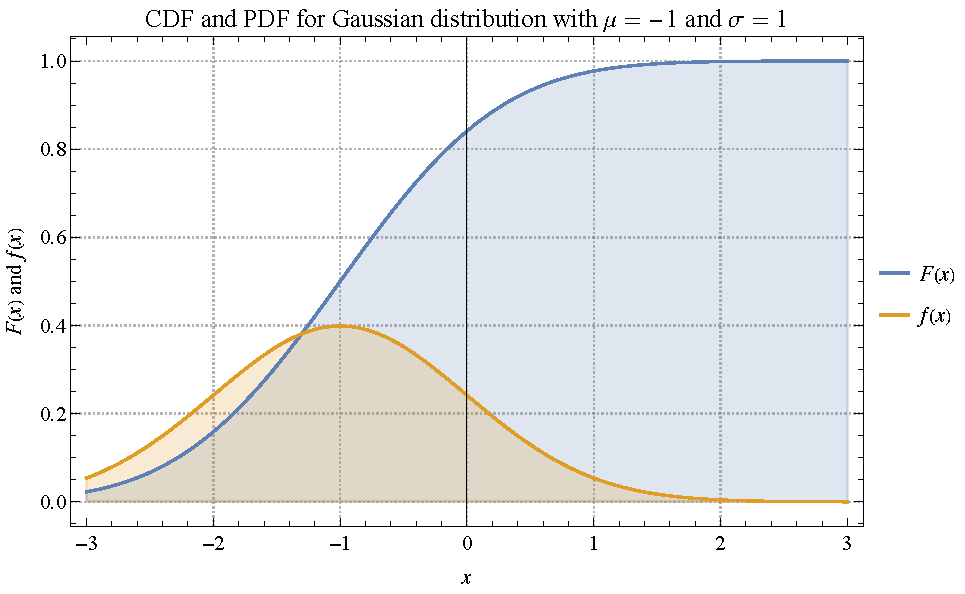
\includegraphics{probability/CDF_PDF_Gaussian.pdf}
	\caption[CDF and PDF for Gaussian distribution.][6pt]{CDF and PDF for Gaussian distribution with $\mu = -1$ and $\sigma = 1$.}
	\label{fig:CDF_PDF_Gaussian}
\end{figure}

\subsection{Probability density function in dim > 1}
\label{subsec:joint_prob_distr}

\begin{equation}
	\frac{\mathrm{d}P}{\mathrm{d}\vec{x}} = f(\vec{x})
\end{equation}

\begin{itemize}[$\to$]
	\item probability density per unit area, volume, $\cdots$
	\item also called “joint probability distribution”\index{joint probability distribution}.
\end{itemize}

\subsection{Marginal distribution}\index{marginal distribution}
\label{subsec:marginal_distr}

\lipsum[8-9]

\subsection{Independent variable}\index{independent variable}
\label{subsec:independent_var}

\lipsum[9-10]

\subsection{Conditional distribution}\index{conditional distribution}
\label{subsec:cond_distr}

\lipsum[10-11]

\subsection{Change of variable}\index{change of variable}
\label{subsec:change_of_var}

\paragraph{Discrete case}\index{change of variable!discrete case}

Take a random variable $x$, and a second variable $y = Y(x)$.

Assume $x$ can take the values $x_{1}, \cdots, x_{n}$, then $y$ can take the values $y_{1} = Y(x_{1}), \cdots, y_{n} = Y(x_{n})$. 

The probability of $y_{i}$ is the sum of the probability of all $x_{i}$ that map into $y_{i}$:

\begin{equation}\label{eq:change_of_var_discrete}
	P(y_{i}) = \sum_{j: \ Y(x_{j})= y_{i}} P(x_{j})
\end{equation}

\paragraph{Continuous case}\index{change of variable!continuous case}

Take a variable $x$ with PDF $f(x)$, and a second variable $y = Y(x)$.

The PDF of $y$ is:

\begin{equation}\label{eq:change_of_var_continuous}
	f(y) = \int {\delta(y - Y(x)) f(x)} \,\mathrm{d}x
\end{equation}

With multiple variables:

\begin{equation}
	f(x’, y’) = \int {\delta(x’ - X(x, y)) \delta(y’ - Y(x, y)) f(x, y)} \,\mathrm{d}x \mathrm{d}y
\end{equation}

If the transformation is invertible, the PDF transforms according to Jacobian determinant\index{Jacobian determinant}:

\begin{equation}
	f(x_{1}, \cdots, x_{n}) = \frac{\mathrm{d}^{n}P’}{\mathrm{d}^{n}x} 
	= \frac{\mathrm{d}^{n}P’}{\mathrm{d}^{n}x’} \left| \det \left(\frac{\partial x’_{i}}{\partial x_{j}} \right) \right|
	= f’(x’_{1}, \cdots, x’_{n}) \left| \det \left(\frac{\partial x’_{i}}{\partial x_{j}} \right) \right|
\end{equation}

In one dimension:

\begin{equation}
	f(x) = f’(x’) \left| \frac{\mathrm{d}x’}{\mathrm{d}x}\right|
	= f(y) \left| \frac{\mathrm{d}y}{\mathrm{d}x}\right|
\end{equation}

\newthought{Example}: \nameref{exer:change_of_var}.



%------------------------------------------------

\section{Expectation operation}\index{expectation}
\label{sec:exp_value}

Let $g(x)$ be some function of a random variable $x$ with density $f(x)$.

The expectation of $g(x)$ is the number:

\marginnote[6pt]{The expectation is a linear operation:

$$
\mathrm{E}\left[ a g(x) + b h(x) \right] = a \mathrm{E}\left( g \right) + b \mathrm{E}\left( h \right)
$$
}

\begin{equation}\label{eq:exp_value}
	\mathrm{E}\left( g \right) = \int_{\Omega} {g(x) f(x)} \,\mathrm{d}x
\end{equation} 

\subsection{Mean or average}\index{mean}\index{average}
\label{subsec:mean}

The average is the expectation of the variable itself:

\begin{equation}\label{eq:mean}
	\left \langle x \right \rangle = \bar{x} = \int {x f(x)}\mathrm{d}x
\end{equation}

In the discrete case:

\begin{equation}\label{eq:mean_discrete}
	\left \langle x \right \rangle = \bar{x} = \sum_{i = 1}^{n}{x_{i} P(x_{i})}
\end{equation}

\subsection{Variance}\index{variance}
\label{subsec:variance}

\begin{equation}\label{eq:variance}
	\mathrm{V} = \mathrm{V}\left( x \right) = \sigma^{2} = \mathrm{E}\left[ (x - \bar{x})^{2} \right] 
	= \int {(x - \bar{x})^{2} f(x)}\mathrm{d}x
	= \left \langle x^{2} \right \rangle - {\left \langle x \right \rangle}^2
\end{equation}

In the discrete case:

\begin{equation}\label{eq:variance_discrete}
	\mathrm{V} = \sum_{i = 1}^{n}{(x_{i} - \bar{x})^{2} P(x_{i})}
\end{equation}

\subsection{Standard deviation}\index{standard deviation}
\label{subsec:std_deviation}

\begin{equation}\label{eq:std_deviation}
	\sigma = \sqrt{\mathrm{V}}
\end{equation}

\subsection{Root mean square}\index{root mean square}
\label{subsec:rms}

\marginnote[6pt]{Sometimes people denote $\sigma$ as $\mathrm{rms}$.}

\begin{equation}\label{eq:rms}
	x_{\mathrm{rms}} = \sqrt{\frac{1}{n}\sum_{i=1}^{n}{{x_{i}}^{2}} P(x_{i})} 
	= \sqrt{\left \langle x^{2} \right \rangle}
\end{equation} 

\subsection{Covariance}\index{covariance}
\label{subsec:cov}

Take two variables $x$, $y$ with PDF $f(x, y)$. The covariance is defined as:

\begin{equation}\label{eq:cov}
	\mathrm{cov}\left( x, y \right) = \mathrm{E}\left[ (x - \bar{x}) (y - \bar{y}) \right] 
	= \mathrm{E}\left( xy \right) - \mathrm{E}\left( x \right) \mathrm{E}\left( y \right) 
\end{equation}

where: 

\begin{equation}
	\mathrm{E}\left( xy \right) = \int {xy f(x, y)}\mathrm{d}x \mathrm{d}y
\end{equation}

\begin{equation}
	\mathrm{E}\left( x \right) = \int {x f(x, y)}\mathrm{d}x \mathrm{d}y
\end{equation}

\subsection{Correlation}\index{correlation}
\label{subsec:corr}

\marginnote[6pt]{Always between -1 and 1.}

\begin{equation}\label{eq:corr}
	\mathrm{corr}\left( x, y \right) = \rho_{x, y} = \frac{\mathrm{cov}\left( x, y \right)}{\sigma_{x} \sigma_{y}}
\end{equation} 

where:

\begin{equation}
	{\sigma_{x}}^{2} = \mathrm{E}\left[ (x - \bar{x})^{2} \right]
\end{equation}

\newthought{If} $x$ and $y$ are independent, we have:

\begin{equation}
	\mathrm{E}\left( xy \right) = \int {xy f_{x}(x) f_{y}(y)}\mathrm{d}x \mathrm{d}y 
	= \int {x f_{x}(x)}\mathrm{d}x \int {y f_{y}(y)}\mathrm{d}y 
	= \mathrm{E}\left( x \right) \mathrm{E}\left( y \right)
\end{equation}

Therefore, \mono{independent variables have null covariance and correlation}.

\newthought{Notice}, however, that uncorrelated variables are not necessarily independent!

This is for example the case (Figure~\ref{fig:uncorrelated_4_Gaussian}) of:

\begin{equation}
	f(x, y) = \frac{1}{4} \left[ 
	g(x; \mu, \sigma) g(y; 0, \sigma) + g(x; -\mu, \sigma) g(y; 0, \sigma)
	+ g(x; 0, \sigma) g(y; \mu, \sigma) + g(x; 0, \sigma) g(y; -\mu, \sigma)
	\right]
\end{equation}

\begin{figure}
	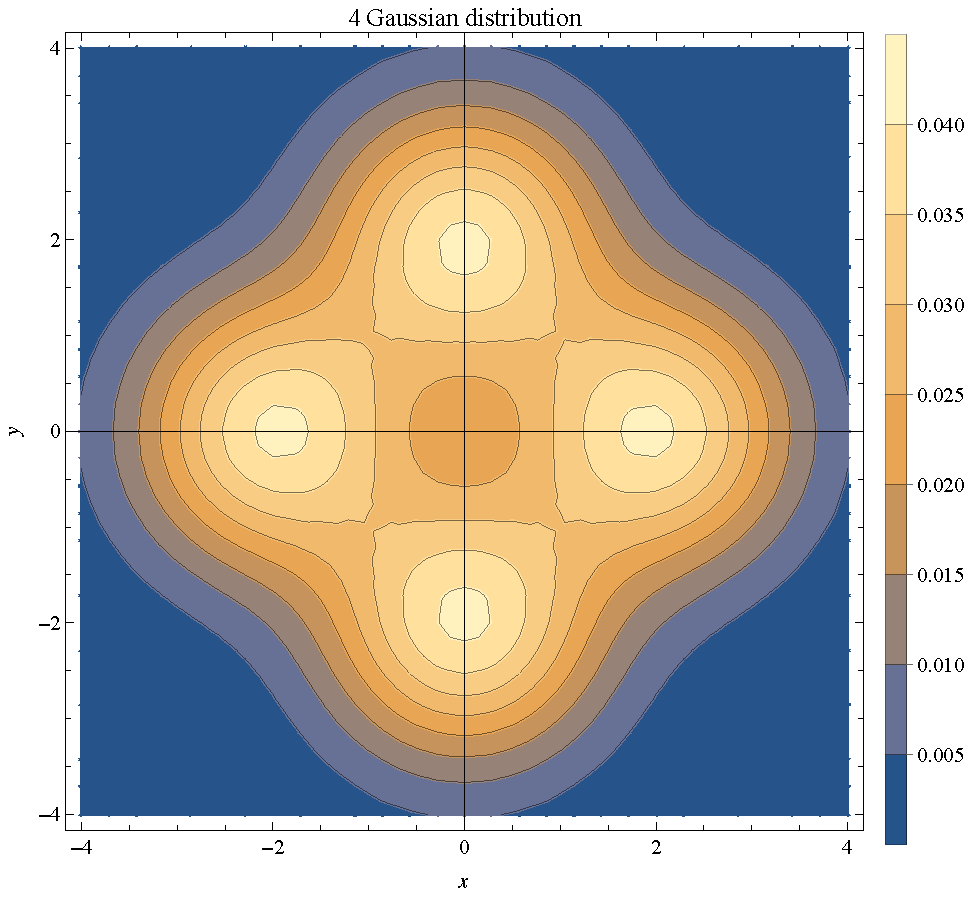
\includegraphics{probability/uncorrelated_4_Gaussian.pdf}
	\caption[4 Gaussian distribution.][6pt]{4 Gaussian distribution.}
	\label{fig:uncorrelated_4_Gaussian}
\end{figure}

\newpage

\subsection{Centroids of a distribution}\index{centroid}
\label{subsec:centroid}

\newthought{Mean}:\index{mean}

\begin{equation}
	\bar{x} = \int {x f(x)}\mathrm{d}x
\end{equation}

\newthought{Mode}:\index{mode}

\begin{equation}\label{eq:mode}
	\hat{x} = \max_{x}(f(x))
\end{equation}

\newthought{Median}:\index{median}

\begin{equation}\label{eq:median}
	\tilde{x} = x: \ P(x < \tilde{x}) = P(x > \tilde{x}) 
	= x: \ \int_{-\infty}^{\tilde{x}} {f(x)} \,\mathrm{d}x 
	= x: \ \int_{\tilde{x}}^{\infty} {f(x)} \,\mathrm{d}x 
	= 0.5
\end{equation}

\newthought{Notice} that mean, mode and median coincide for a symmetric distribution, but \emph{not} for an asymmetric one! (Figure~\ref{fig:mean_mode_median_chisquare})

\begin{figure*}[h]\index{chi-square distribution}
	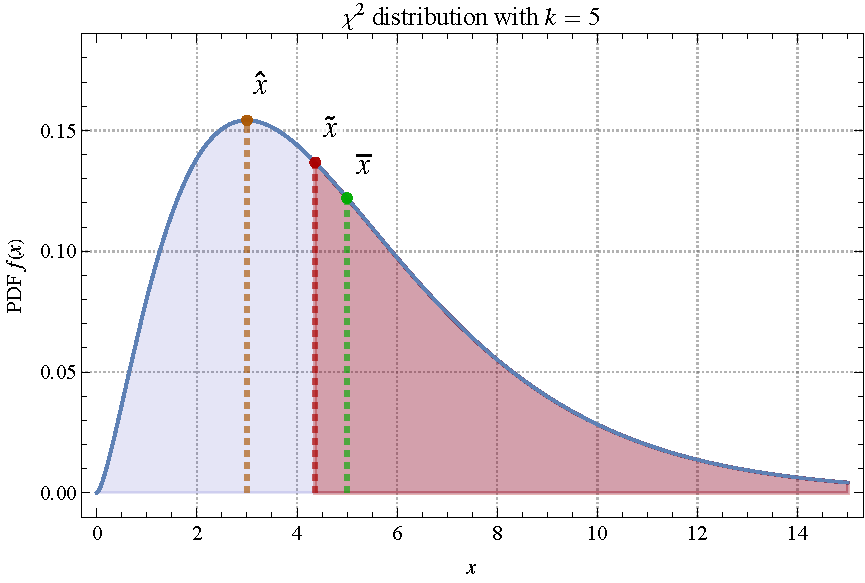
\includegraphics[width=\linewidth]{probability/mean_mode_median_chisquare.pdf}
	\caption[$\chi^{2}$ distribution with $k = 5$.]{$\chi^{2}$ distribution with $k = 5$.}
	\label{fig:mean_mode_median_chisquare}
\end{figure*}

\subsection{Quantiles}\index{quantile}
\label{subsec:quantile}

The quantity $q_{\alpha}$ such that:

\begin{equation}\label{eq:alpha_quantile}
	\int_{-\infty}^{q_{\alpha}} {f(x)} \,\mathrm{d}x = \alpha 
	= 1 - \int_{q_{\alpha}}^{\infty} {f(x)} \,\mathrm{d}x
\end{equation}

is called $\alpha$-quantile.

An alternative definition can be given with the cumulative distribution\index{cumulative distribution}:

\begin{equation}
	q_{\alpha} = x : \ F(x) = \alpha
\end{equation}


%------------------------------------------------

\section{Distribution}\index{distribution}
\label{sec:distr}

\subsection{Bernoulli distribution}\index{Bernoulli distribution}
\label{subsec:Bernoulli_distr}

The distribution is expressed by:

\begin{equation}\label{eq:Bernoulli_distr}
	f(k ; p) = \left\{
	\begin{array}{lcl}
		p     & & {\textrm{if } k = 1}\\
		1 - p & & {\textrm{if } k = 0}
	\end{array} \right.
	= p^{k}(1-p)^{1 - k} \quad \textrm{for } k \in \{ 0, 1 \}
\end{equation}

\begin{itemize}
	\item Mean: $\bar{x} = \sum_{x = 0}^{1} {x f(x ; p)}  = 1 \cdot f(1 ; p) = p$
	\item $\left \langle x^{2} \right \rangle = p$
	\item Variance: $\mathrm{V} = \left \langle x^{2} \right \rangle - {\bar{x}}^{2} = p(1 - p)$
\end{itemize}

\subsection{Binomial distribution}\index{binomial distribution}
\label{subsec:binomial_distr}

\begin{equation}\label{eq:binomial_distr}
	P(k ; n, p) = \frac{n!}{k!(n-k)!} p^{k}(1-p)^{n - k}
\end{equation}

\begin{itemize}
	\item Mean: $\bar{k} = np$
	\item Variance: $\mathrm{V} = np(1 - p)$
\end{itemize}

\newthought{Exercise}: \nameref{exer:binomial_distr}.

\subsection{Multinomial distribution}\index{multinomial distribution}
\label{subsec:multinomial_distr}

\marginnote{An example of multinomial distribution is a histogram containing $n$ entries distributed in $m$ bins.}

\begin{equation}\label{eq:multinomial_distr}
	P(k_{1}, k_{2}, \cdots, k_{m} ; n, p_{1}, \cdots, p_{m}) 
	= \frac{n!}{k_{1}! \cdots k_{m}!} {p_{1}}^{k_{1}} {p_{2}}^{k_{2}} \cdots {p_{m}}^{k_{m}}
\end{equation}

\begin{itemize}
	\item Average: $\overline{k_{i}} = n {p}_{i}$
	\item Variance: $\mathrm{V}\left[ k_{i} \right] = n {p}_{i} (1 - {p}_{i})$
	\item Covariance: $\mathrm{cov}\left( k_{i}, k_{j} \right) = - n {p}_{i} {p}_{j} \quad \forall i \neq j$
\end{itemize}

\subsection{Uniform distribution}\index{uniform distribution}
\label{subsec:uniform_distr}

A variable $x$ is uniformly distributed in the interval $[a, b)$, if its PDF (Figure~\ref{fig:CDF_PDF_uniform}) is constant in such range, \ie:

\begin{equation}\label{eq:uniform_distr}
	f(x) = \left\{
	\begin{array}{ccl}
		\frac{1}{b - a} & & {\textrm{if } a \leq x < b}\\
		0 & & {\textrm{otherwise}}
	\end{array} \right.
\end{equation}

\begin{figure}
	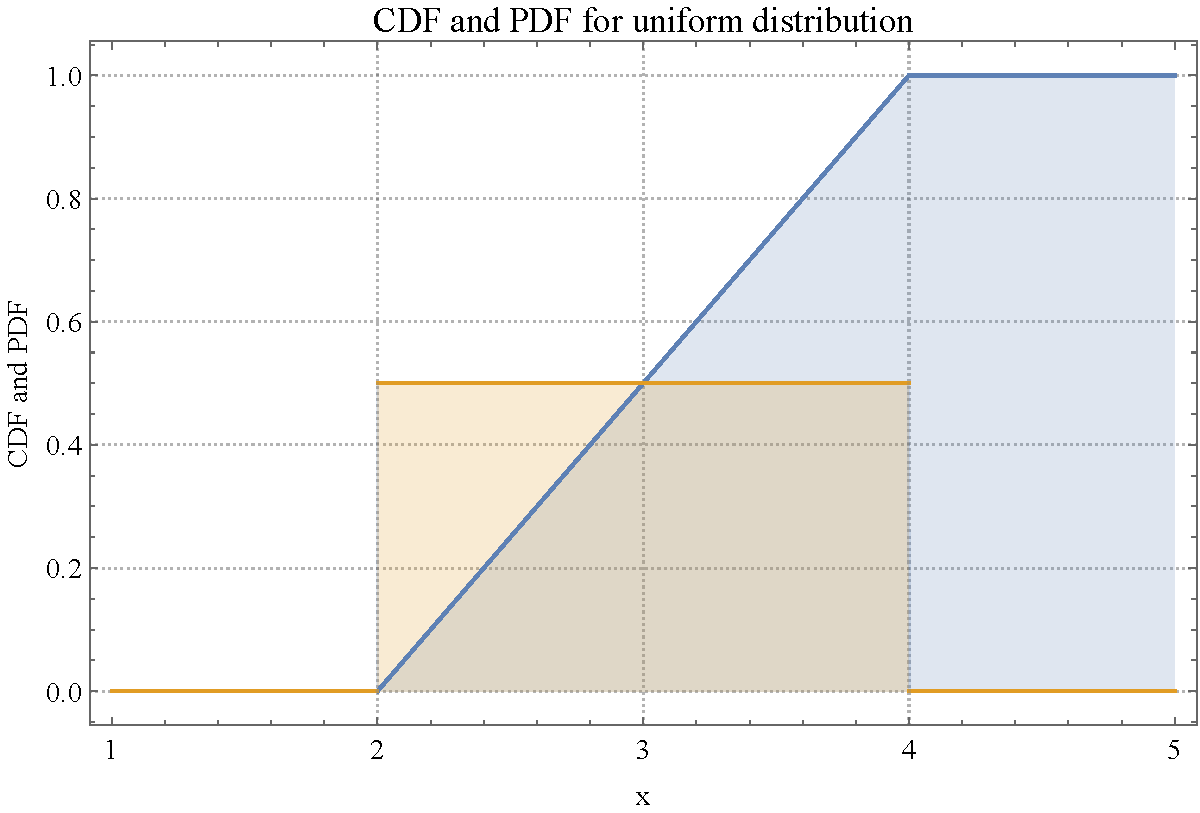
\includegraphics{probability/CDF_PDF_uniform.pdf}
	\caption[CDF and PDF for uniform distribution.][6pt]{CDF and PDF for uniform distribution.}
	\label{fig:CDF_PDF_uniform}
\end{figure}

\begin{itemize}
	\item Average: $\bar{x} = \frac{a + b}{2}$
	\item Standard deviation: $\sigma = \frac{b - a}{\sqrt{12}}$
\end{itemize}

\subsection{Exponential distribution}\index{exponential distribution}
\label{subsec:expo_distr}

Take a variable $x \geq 0$, and a constant $\lambda > 0$.

An exponential distribution (Figure~\ref{fig:CDF_PDF_expo}) has the form:

\begin{equation}\label{eq:expo_distr}
	f(x ; \lambda) = \lambda \mathrm{e}^{- \lambda x}
\end{equation}

\begin{figure}
	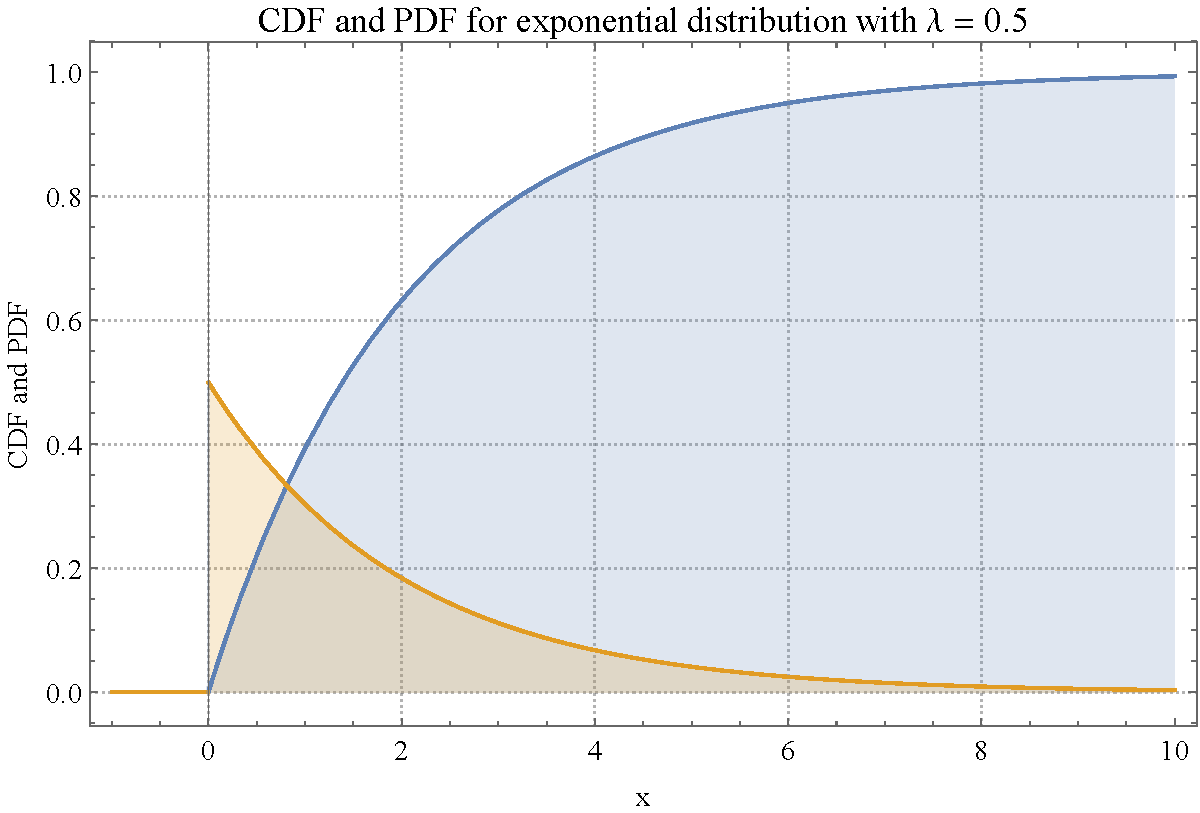
\includegraphics{probability/CDF_PDF_expo.pdf}
	\caption[CDF and PDF for exponential distribution.][6pt]{CDF and PDF for exponential distribution with $\lambda = 0.5$.}
	\label{fig:CDF_PDF_expo}
\end{figure}

\begin{itemize}
	\item Average: $\bar{x} = \frac{1}{\lambda}$
	\item Standard deviation: $\sigma = \frac{1}{\lambda}$
\end{itemize}

\newthought{Exercise}: \nameref{exer:expo_from_uniform}!

\subsection{Poisson distribution}\index{Poisson distribution}
\label{subsec:poisson_distr}

Consider a uniformly distributed variable $t$ over an interval $[0, \Delta t]$.

\marginnote{$t$ could be a space or a time variable, like the coordinate of some particle bit on a pixelated detector, or the time of arrival of some particles.}

Assume $t$ is extracted $n$ times in $\Delta t$, the rate of extractions is $r = \frac{n}{\Delta t}$.

Let's consider only the extractions $k$ in a shorter interval $\delta t$, which are clearly binomial distributed. 

Assume $n$ and $\Delta t$ are constant, and take the limits $n \to \infty$ and $\Delta t \to \infty$, keeping their ratio $r$ fixed.

The expected value $\nu$ of the number of extractions in $\delta t$ is:

$$
\nu = \left \langle k \right \rangle = \frac{n}{\Delta t} \delta t = r \delta t
$$

And $k$ follows a binomial:

$$
P(k ; n, \nu) = \frac{n!}{k!(n-k)!} {\left( \frac{\nu}{n} \right)}^{k} {\left( 1 - \frac{\nu}{n} \right)}^{n - k}
$$

with $\lim_{n \to \infty}$:

$$
P(k ; n, \nu) 
= \frac{\nu^{k}}{k!} 
\cdot \underset{\to 1}{\underbrace{\frac{n(n - 1) \cdots (n - k + 1)}{n^{k}}}}  
\cdot \underset{\to \mathrm{e}^{- \nu}}{\underbrace{{\left( 1 - \frac{\nu}{n} \right)}^{n}}} 
\cdot \underset{\to 1}{\underbrace{{\left( 1 - \frac{\nu}{n} \right)}^{- k}}}
$$

We have then the Poisson distribution:

\begin{equation}\label{eq:poisson_distr}
	P(k ; \nu) = \frac{\nu^{k} \mathrm{e}^{- \nu}}{k!}
\end{equation} 

\begin{itemize}
	\item Average: $\bar{k} = \nu$
	\item Standard deviation: $\sigma = \sqrt{\nu}$
\end{itemize}

\newthought{Exercise}: \nameref{exer:poisson_distr}.

\subsection{Properties of Poisson distribution}\index{Poisson distribution!property}
\label{subsec:prop_of_poisson_distr}

\begin{itemize}
	\item For large $\nu$, a Poisson distribution can be approximated with a Gaussian\index{Gaussian distribution} with $\mu = \nu$ and $\sigma = \sqrt{\nu}$.
	\item A binomial distribution\index{binomial distribution} with $p \ll 1$ can be approximated with a Poisson distribution with $\nu = np$.
	\item If two variables $k_{1}$ and $k_{2}$ are Poisson distributed with expectation values $\nu_{1}$ and $\nu_{2}$, their sum $k = k_{1} + k_{2}$ is Poisson distributed with expectation value $\nu = \nu_{1} + \nu_{2}$. (Figure~\ref{fig:prop_of_Poisson_distr}) 
		\marginnote[-6pt]{This can be expanded to any number of Poisson variables.}
	\item Randomly picking with probability $\varepsilon$ from a Poisson process gives again a Poisson process.
		\marginnote[-6pt]{This is the case of a detector with efficiency $\varepsilon$, which measures a Poisson process with expectation value $\nu_{0}$!}
		\begin{description}
			\item Take a Poisson variable $n_{0}$ with expectation value $\nu_{0}$. 
			\item Then a binomial variable $k$ with probability $\varepsilon$ and sample size $n_{0}$ is distributed as a Poisson with average $\nu = \varepsilon \nu_{0}$.
		\end{description}
\end{itemize}

\begin{figure}
	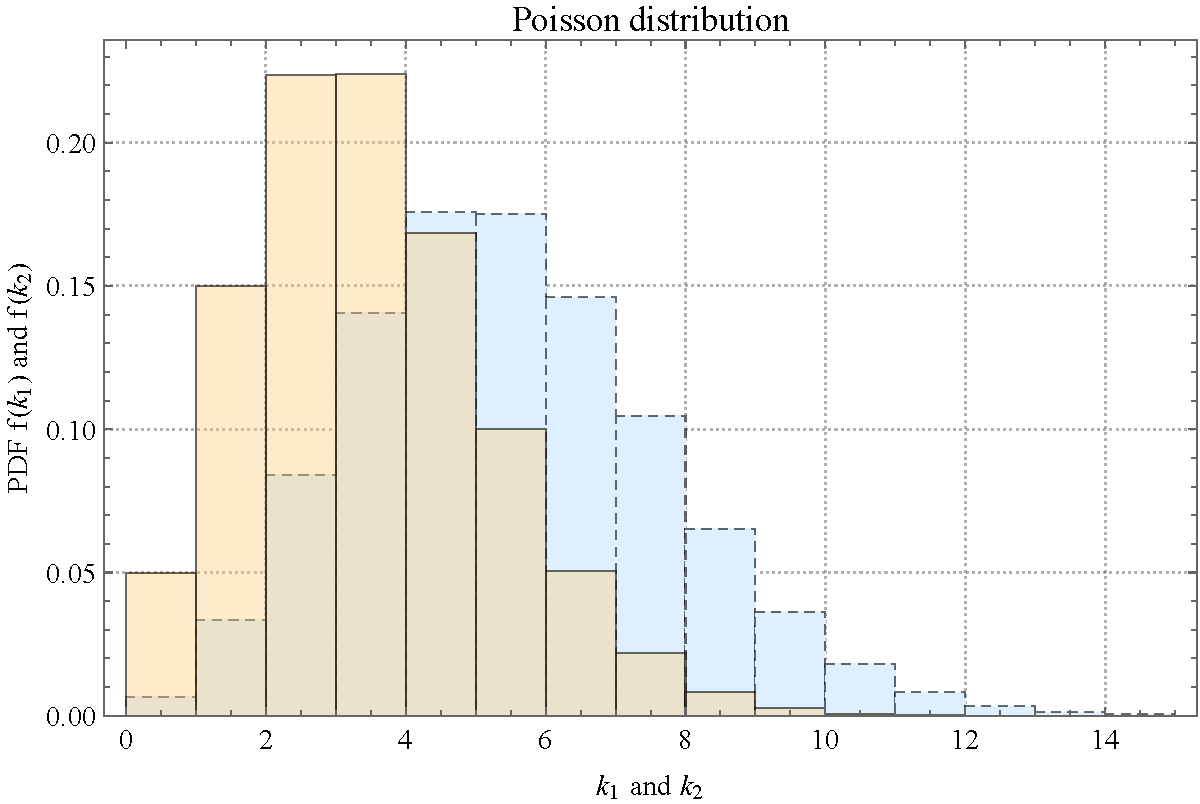
\includegraphics{probability/prop_of_Poisson_distr.pdf}
	\caption[PDF for two Poisson distributions.][6pt]{PDF for two Poisson distributions.}
	\label{fig:prop_of_Poisson_distr}
\end{figure}

\newthought{Examples}:

Suppose you have $n$ unstable isotopes, with decay rate $\lambda$ (numbers of decays per unit time).

In a time $\Delta t$, the probability of a decay is $p = \lambda t$.

The distribution of the numbers of decayed nuclei in a time $\Delta t$ is:

\begin{enumerate}
	\item Binomial, if $p \gtrsim 0.1$
	\item Poisson, if $p \lesssim 0.1$
\end{enumerate}

\begin{table}
	\centering
	\begin{tabular}{l c c}
		\toprule
		& ${}^{137}\mathrm{Cs}$ & ${}^{82}\mathrm{Rb}$\\
		\midrule
		Decay mode 
		& $\beta -$ & EC $\beta +$\\
		Half-life $T_{1/2}$ 
		& $\unit[30.08]{y}$ & $\unit[75.45]{s}$\\
		Decay rate $\lambda$ $[\unit{s}^{-1}]$ 
		& $7.3 \times 10^{-10}$ & $9.2 \times 10^{-3}$\\
		Radioactive activity $A$ $[\unit{Ci}]$ 
		& $1 \mu \unit{Ci}$ & $\unit[1]{m Ci}$\\
		Radioactive activity $A$ $[\unit{Bq}]$ 
		& $3.7 \times 10^{4}$ & $3.7 \times 10^{7}$\\
		\tabincell{l}{Initial amount of active substance \\ $N_{0} = \frac{A}{\lambda}$} & $5.1 \times 10^{13}$   & $4 \times 10^{9}$      \\
		\tabincell{l}{Number of decay events in 1 hour \\ $\Delta N = N_{0} \times \lambda \times \Delta t$} & $1.3 \times 10^{8} \ll N_{0}$ & $1.3 \times 10^{11} {\color{Red} > N_{0}}$\\
		\bottomrule
	\end{tabular}
	\caption[Binomial or Poisson?]{Binomial or Poisson for measuring decays over 1 hour?}
	\label{tab:binomial_or_poisson}
\end{table}

\subsection{Normal (Gaussian) distribution}\index{Gaussian distribution}
\label{subsec:gaussian_distr}

\begin{equation}\label{eq:gaussian_distr}
	g(x ; \mu, \sigma) = \frac{1}{\sigma \sqrt{2 \pi}} 
	\mathrm{e}^{- \frac{1}{2} {\left( \frac{x - \mu}{\sigma} \right)}^{2}}
\end{equation}

with $x$ continuous. 

For $\mu = 0$ and $\sigma = 1$, we have a standard normal distribution\index{standard normal distribution}:

\begin{equation}\label{eq:std_normal_distr}
	\phi(x) = \frac{1}{\sqrt{2 \pi}} \mathrm{e}^{- \frac{x^{2}}{2}}
\end{equation}

\begin{itemize}
	\item Mean: $\mu$
	\item Standard deviation: $\sigma$
\end{itemize}

Cumulative of standard normal:

\begin{equation}\label{eq:cdf_std_normal}
	\Phi(x) = \frac{1}{\sqrt{2 \pi}} \int_{-\infty}^{x} \mathrm{e}^{- \frac{y^{2}}{2}} \,\mathrm{d}y 
	= \frac{1}{2} \left[ \mathrm{erf}\left( \frac{x}{\sqrt{2}} \right) + 1 \right]
\end{equation}

Cumulative of Gaussian:

\begin{equation}\label{eq:cdf_Gaussian}
	G(x ; \mu, \sigma) = \Phi \left( \frac{x - \mu}{\sigma} \right) 
	= \frac{1}{2} \left[ \mathrm{erf}\left( \frac{x - \mu}{\sigma \sqrt{2}} \right) + 1 \right]
\end{equation}

\subsection{Properties of Gaussian distribution}\index{Gaussian distribution!property}
\label{subsec:prop_of_gaussian_distr}

If $x_{1}$ and $x_{2}$ are Gaussian distributed with means $\mu_{1}$, $\mu_{2}$ and standard deviations $\sigma_{1}$, $\sigma_{2}$, their combination $x = a{x}_{1} + b{x}_{2}$ is Gaussian distributed with mean $\mu = a{\mu}_{1} + b{\mu}_{2}$ and standard deviation $\sigma = \sqrt{a^{2}{{\sigma}_{1}}^{2} + b^{2}{{\sigma}_{2}}^{2}}$.

\marginnote[-6pt]{Sometimes the sum of two Gaussian distributed variables is not a Gaussian! \nameref{exer:sum_of_Gaussian}.}

\subsection{Multivariate normal distribution}\index{multivariate normal distribution}
\label{subsec:multivariate_normal_distr}

A multivariate normal distribution is a Gaussian in dim > 1.

\paragraph{Dim = 2}

\begin{equation}\label{eq:bivariate_normal_joint_density}
	g(x, y) = \frac{1}{\sqrt{2 \pi {\left| C \right|}}} \mathrm{e}^{\left[ - \frac{1}{2} (x, y) C^{-1} 
	\left( \begin{array}{c}
		x \\
		y 
	\end{array} \right) \right]}
\end{equation}

where $C$ is the covariance matrix\index{covariance matrix}: 

\begin{equation}\label{eq:covariance_matrix}
	C = 
	\left( \begin{array}{cc}
		{\sigma_{x}}^{2} & \rho_{xy} \sigma_{x} \sigma_{y} \\
		\rho_{xy} \sigma_{x} \sigma_{y} & {\sigma_{y}}^{2}
	\end{array} \right)
\end{equation}

One can also forget about the covariance matrix and define a rotation of the system of reference: 

\begin{equation}\label{eq:rotation_of_system_of_reference}
	\left\{
	\begin{array}{l}
		x' = \cos \phi \cdot x + \sin \phi \cdot y\\
		y' = - \sin \phi \cdot x + \cos \phi \cdot y
	\end{array} \right.
\end{equation}

therefore, 

\begin{equation}
	g(x', y') = \frac{1}{2 \pi \sigma_{1} \sigma_{2}} 
	\mathrm{e}^{- \frac{1}{2} {\left( \frac{x' - \mu_{1}}{\sigma_{1}} \right)}^{2}} 
	\mathrm{e}^{- \frac{1}{2} {\left( \frac{y' - \mu_{2}}{\sigma_{2}} \right)}^{2}}
\end{equation}

\marginnote[-6pt]{By importing the rotation, one can get rid of the correlation.}

\paragraph{General formula for dim = $n$}

\begin{equation}\label{eq:bivariate_normal_joint_density}
	g(\vec{x}) = \frac{1}{\sqrt{(2 \pi)^{n} {\left| C \right|}}} 
	\mathrm{e}^{\left[ - \frac{1}{2} (\vec{x} - \vec{\mu})^{T} C^{-1} (\vec{x} - \vec{\mu}) \right]}
\end{equation}

\subsection{Chi-square distribution}\index{chi-square distribution}
\label{subsec:chisquare_distr}

A $\chi^{2}$ random variable with $n$ degrees of freedom is the sum of $n$ standard normal variables.

\begin{equation}\label{eq:chisquare_distr}
	f(\chi^{2} ; n) = \frac{2^{- \frac{n}{2}}}{\Gamma(\frac{n}{2})} \chi^{n - 2} \mathrm{e}^{- \frac{\chi^{2}}{2}}
\end{equation}

where $\Gamma$ is the gamma function\index{gamma function}, which is the extension of the factorial\index{factorial}.

\marginnote[-6pt]{For integer, $\Gamma(n) = (n -1)!$ .}

\begin{itemize}
	\item Expectation value: $\left \langle \chi^{2} \right \rangle = n$
	\item Standard deviation: $\sigma = \sqrt{2n}$
\end{itemize}

\newthought{Exercise}: \nameref{exer:chisquare_distr}.




%----------------------------------------------------------------------------------------
%	MONTE CARLO METHODS
%----------------------------------------------------------------------------------------

\chapter{Monte Carlo methods}
\label{ch:monte_carlo}


%------------------------------------------------

\section{Theorems in statistics}
\label{sec:theorem_in_stat}

\subsection{Convergence in probability}\index{convergence in probability}
\label{subsec:convergence_in_prob}

The sequence $\{ x_{1}, \cdots, x_{n} \}$ is said to converge in probability to $\bar{x}$ (Figure~\ref{fig:convergence}) if $\forall \epsilon > 0$ and $\forall \eta > 0$, a value $n_{0}$ can be found such that:

\begin{equation}\label{eq:convergence_in_prob}
	P(|x_{n} - \bar{x}| > \varepsilon) < \eta \quad \forall n \geq n_{0}
\end{equation}

\begin{figure}
	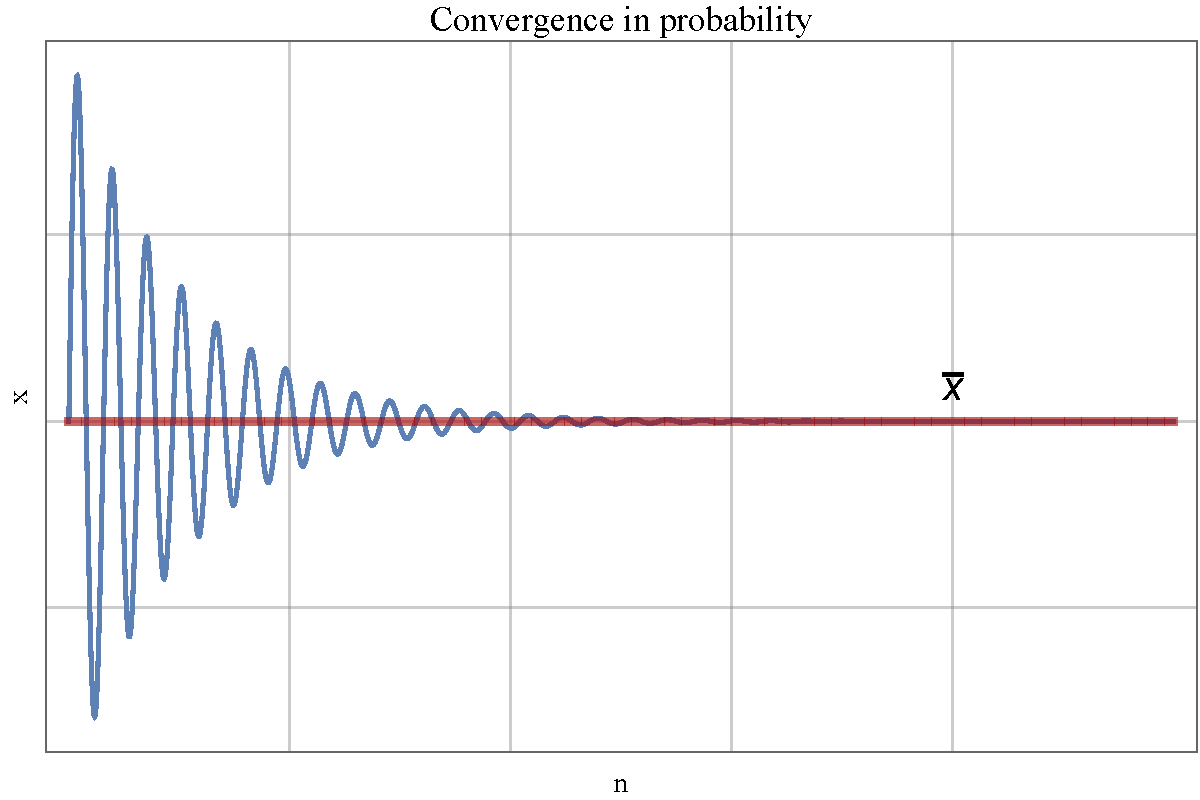
\includegraphics{monte_carlo/convergence.pdf}
	\caption[Convergence in probability.][6pt]{Convergence in probability.}
	\label{fig:convergence}
\end{figure}

\subsection{Law of large number}\index{law of large number}
\label{subsec:law_of_large_number}

Assume to repeat the same measurement $n$ times, where outcome is a random variable $x$ with a given PDF and STD $\sigma$.

The average will be:

\begin{equation}\label{eq:average}
	\bar{x} = \frac{1}{n} \sum_{i = 1}^{n}{x_{i}}
\end{equation}

\begin{itemize}[$\to$]
	\item \newthought{Weak law}\index{law of large number!weak law}: If the mean $\mu$ exists, and if $\lim_{n \to \infty} \left[ \frac{1}{n^{2}} \sum_{i} {\sigma_{i}}^{2} \right] = 0$, then $\bar{x}$ converges to $\mu$ in quadratic mean: $\lim_{n \to \infty} {\mathrm{E}\left[ (\bar{x} - \mu)^{2} \right]} = 0$.
	\item \newthought{Strong law}\index{law of large number!strong law}: If $\lim_{n \to \infty} \left[ \sum_{i} {\left( \frac{\sigma_{i}}{i} \right) }^{2} \right]$ is finite, then $\bar{x}$ converges almost certainly to $\mu$, which means that $P\left(\lim_{n \to \infty} {\bar{x}} = \mu \right) = 1$.
\end{itemize}

\marginnote[-6pt]{Take home message: if the parent mean $\mu$ exists, the more you measure, the closer the sample mean $\bar{x}$ will go to $\mu$.}

\subsection{Central limit theorem}\index{central limit theorem}
\label{subsec:central_limit_theorem}

Recall that if we have a sequence of independent variable $x_{i}$, each with  a distribution with mean $\mu_{i}$ and variance ${\sigma_{i}}^{2}$, the distribution of the sum $s = \sum_{i}{x_{i}}$ will have mean $\mu = \sum_{i}{\mu_{i}}$ and variance $\sigma^{2} = \sum_{i}{{\sigma_{i}}^{2}}$. 

The central limit theorem states that:

\begin{equation}\label{eq:central_limit_theorem}
	\lim_{n \to \infty} {\frac{s - \sum_{i = 1}^{n}{\mu_{i}}}{\sqrt{\sum_{i = 1}^{n}{{\sigma_{i}}^{2}}}} } = \mathrm{Gaus}(0, 1)
\end{equation}

In other words, sum of $n$ random variables tend to a Gaussian.

\marginnote{Or, as Shihong said, “the end of the World is Gaussian”.}

\newthought{Example}: \nameref{exer:gaussian_random_number_generator}.



%------------------------------------------------

\section{Pseudorandom numbers and Monte Carlo methods}
\label{sec:pseudorandom_number}

\subsection{Pseudorandom number generator}\index{pseudorandom number}
\label{subsec:pseudorandom_number_generator}

So far, we have used random numbers in almost all exercises, without actually explaining what they are and what are their properties and limitations. 

A pseudorandom number generator is an algorithm that generates a sequence of numbers distributed according to some PDF and that resemble very closely an actual distribution of random numbers with the same PDF.

\subsection{Properties of pseudorandom number generator}\index{pseudorandom number!property}
\label{subsec:prop_of_pseudorandom_number_generator}

\begin{itemize}[$\to$]
	\item Each extraction must be statistically independent from previous ones: $f(x_{i} \mid x_{i - m}) = f(x_{i}) \quad \forall i, m$.
	\item All extraction should be distributed according to the same PDF: $f(x_{i}) = f(x_{j}) \quad \forall i, j$.
	\item after a given period $p$, the sequence will repeat itself: $x_{i + p} = x_{i}$.
		\marginnote{Obviously, we want $p$ to be as large as possible.}
		\begin{description}
			\item In this sense, the distribution of $n$ pseudorandom numbers can be consider to be truly random up to $n = p$.
		\end{description}
	\item We should be albe to initialize the generator in such a way that it can reproduce exactly the same sequence of random numbers.
		\marginnote{This is very useful for debugging code.}
		\begin{description}
			\item The initialization is commonly done by passing a user-defined number called seed.
		\end{description}
\end{itemize}

\subsection{Uniform random number generator}\index{uniform random number}
\label{subsec:uniform_random_number_generator}

Most common and simple generator produces numbers in $[0, 1)$.

For example, the \doccmddef{lrand48()} (standard of \mono{C}) uses the following algorithm:

\begin{equation}\label{eq:lrand48}
	x_{i + 1} = (a x_{i} + c) \mod(m)
\end{equation}

where: $m = 2^{48}, a = 25 \ 214 \ 903 \ 917, c = 11$.

The produced random numbers are uniformly distributed between $0$ and $2^{48} - 1$, and mapped into floating-point numbers between $0$ and $1$.

\begin{itemize}[$\to$]
	\item A uniform random number can be remapped to any other interval $[a, b)$ simply by doing: $x \to x' = a + x(b - a)$.
\end{itemize}

\subsection{Non-uniform random number generator}\index{non-uniform random number}
\label{subsec:non_uniform_random_number_generator}

\paragraph{Inverse-transformation method}

Suppose we want to generate a random number distributed as $f(x)$.

The cumulative $F(x)$ will map $x \to [0, 1)$.

Therefore, we can invert (analytically or numerically) $F(x)$ to obtain a number distributed as $f(n)$.

\begin{enumerate}
	\item Generate $r$ uniformly in $[0, 1)$.
	\item Invert $F$: $x = F^{-1}(r)$. (Figure~\ref{fig:inverse_transformation_method})
\end{enumerate}

\begin{figure}
	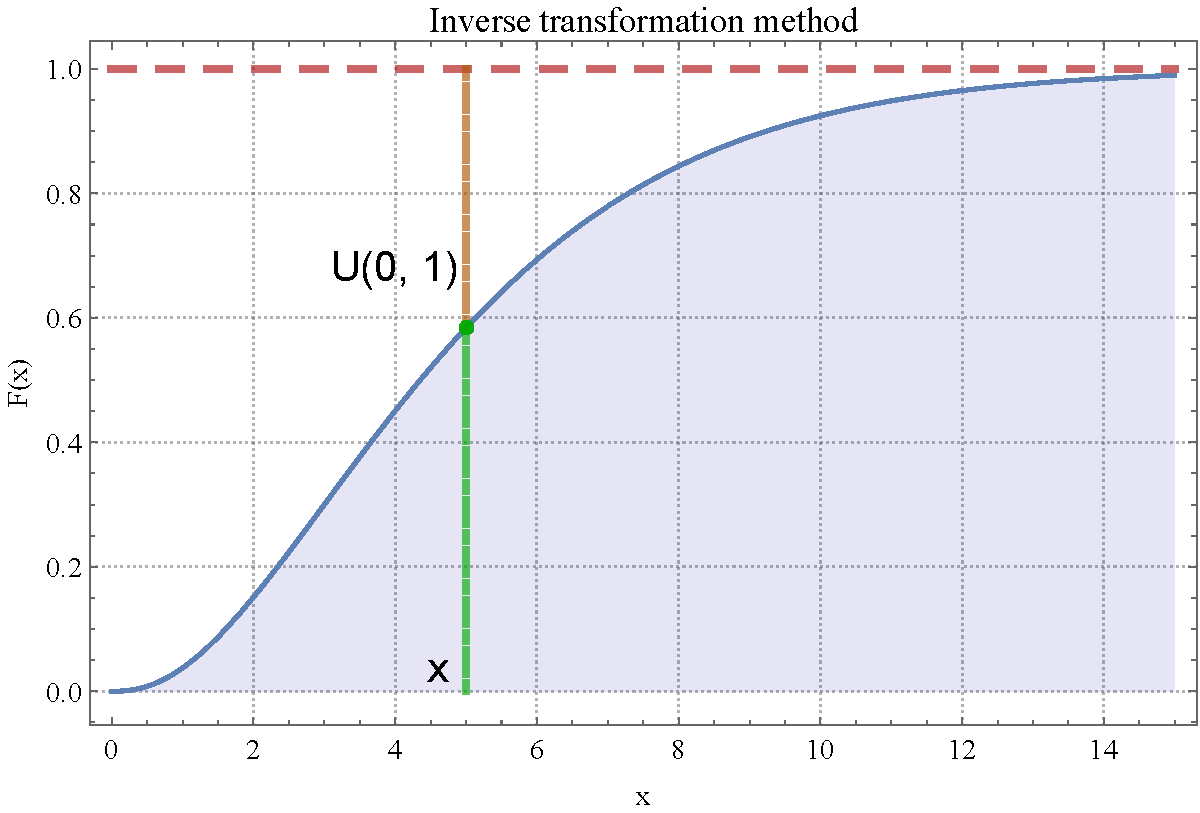
\includegraphics{monte_carlo/inverse_transformation_method.pdf}
	\caption[Inverse-transformation method.][6pt]{Generate non-uniform random number by using inverse-transformation method.}
	\label{fig:inverse_transformation_method}
\end{figure}

\subsection{Gaussian generator using central limit theorem}
\label{subsec:gaussian_generator}

$\to$ It works, but

\begin{enumerate}
	\item It is \mono{fucking} inefficient.
	\item It is truncated.
\end{enumerate}

\newthought{Exercise}: \nameref{exer:gaussian_random_number_generator}.

\subsection{Acceptance-rejection method (hit-or-miss method)}\index{acceptance-rejection}\index{hit-or-miss}
\label{subsec:acceptance_rejection}

Assume a PDF $f(x)$ defined in interval $[x_{1}, x_{2})$.

Assume we know $m = \max \left\{ f(x), x \in [x_{1}, x_{2}) \right\}$.

Then we can do the following:

\begin{enumerate}
	\item Generate a uniform number $x$ in $[x_{1}, x_{2})$.
	\item Generate a uniform number $r$ in $[0, m)$.
	\item If $f(x) > r$, we accept $x$, otherwise, we go back to 1. . (Figure~\ref{fig:acceptance_rejection})
	\item Populate a histogram with the accepted values. This will approximate the original $f(x)$ for large number of generated points.
\end{enumerate}

\begin{figure}
	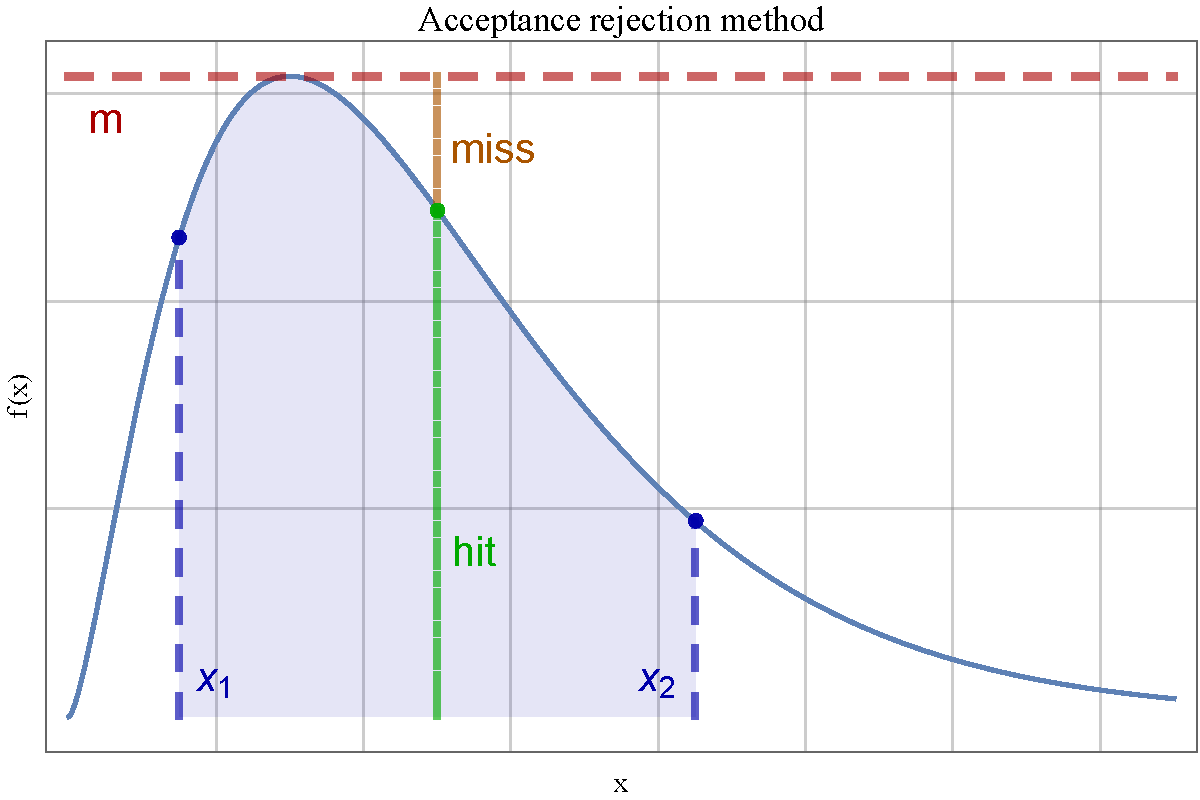
\includegraphics{monte_carlo/acceptance_rejection_method.pdf}
	\caption[Acceptance-rejection method.][6pt]{Generate non-uniform random number by using acceptance-rejection method.}
	\label{fig:acceptance_rejection}
\end{figure}

\subsection{Properties of acceptance-rejection method}\index{acceptance-rejection!property}
\label{subsec:prop_of_acceptance_rejection}

\begin{itemize}[$\to$]
	\item The method works well if we can compute $f(x)$ fast enough, but if $F(x)$ is computationally intensive.
	\item We only get a binned approximation of $f(x)$.
	\item The efficiency of the method is:
		$$
		\varepsilon = \frac{\int_{x_{1}}^{x_{2}}{f(x)} \,\mathrm{d}x}{(x_{2} - x_{1}) \cdot m}
		$$
		Therefore, it is inefficient if $f(x)$ is very peaked.
	\item It can be applied to multi-dimensional cases, but leads to the “curve of dimensionality”.
\end{itemize}

\newthought{Example}: \nameref{exer:acceptance_rejection}.

\subsection{Combination of random variables}
\label{subsec:combination_of_random_var}

For complicated cases, we can combine the inverse-transformation method and the acceptance-rejection method.

We can also use random number generator to produce binned PDFs of variables that are a combination of other variables.

This is for example the case of the ratio of two variables.

\newthought{Example}: \nameref{exer:change_of_var}.



%------------------------------------------------

\section{Numerical algorithms with Monte Carlo}\index{Monte Carlo method}
\label{sec:numerical_monte_carlo}

\subsection{Numerical integration with Monte Carlo}\index{numerical integration}
\label{subsec:numerical_int}

The acceptance-rejection method estimates the integral $\int_{x_{1}}^{x_{2}}{f(x)} \,\mathrm{d}x$ from the fraction of accepted events $k$ over the number $n$ of generated events:

\begin{equation}\label{eq:numerical_int}
	I = \int_{x_{1}}^{x_{2}}{f(x)} \,\mathrm{d}x \simeq (x_{2} - x_{1}) \cdot m \cdot \frac{k}{n}
\end{equation}

The uncertainty is (we will see it in some future lecture):

\begin{equation}\label{eq:uncertainty_of_numerical_int}
	\sigma_{\hat{I}} = \sqrt{\frac{\hat{I} \left[ (x_{2} - x_{1}) \cdot m - \hat{I} \right]}{n}}
\end{equation}

Notice that there is no dependence on the dimensionality.

This makes Monte Carlo method advantageous when computing the integral of high-dimensionality PDFs.

The problem, however, might be to find the maximum of $f(x)$.

\subsection{Markov chain Monte Carlo}\index{Markov chain Monte Carlo}
\label{subsec:mcmc}

Some probability distributions can be sampled more efficiently by producing sequence of correlated pseudorandom number, where each $x_{i}$ depends on the previous $m$ extractions.

A sequence of random variables $x_{0}, x_{1}, \cdots, x_{n}$ is a Markov chain if the PDF obeys to:

\begin{equation}\label{eq:mcmc_pdf}
	f(x_{n + 1} ; x_{0}, \cdots, x_{n}) = f(x_{n + 1} ; x_{n})
\end{equation}

\ie, if $f(x_{n + 1})$ depends only on the immediately previous extraction.

This works in any dimension.

\subsection{Metropolis–Hastings algorithm}\index{Metropolis–Hastings algorithm}
\label{subsec:metropolis}

A common Markov chain Monte Carlo algorithm is Metropolis–Hastings algorithm.

Suppose we want to sample a PDF $f(\vec{x})$. We do the following:

\begin{enumerate}
	\item Pick a point $\vec{x}_{0}$ uniformly distributed in the sample space $\Omega$.
	\item Evaluate $f(\vec{x}_{0})$.
	\item Generate a second point $\vec{x}$ according to a predefined PDF $q(\vec{x}, \vec{x}_{0})$, called “proposal distribution”.
	\item Evaluate $f(\vec{x})$.
	\item Generate a uniform number $u \in [0, 1)$.
	\item If
		$$
		\frac{f(\vec{x}) q(\vec{x}_{0}, \vec{x})}{f(\vec{x}_{0}) q(\vec{x}, \vec{x}_{0})} > u
		$$
		accept the point and set $\vec{x}_{1} = \vec{x}$. Otherwise, reject $\vec{x}$.
		\marginnote{Notice that: if $q(\vec{x}, \vec{x}_{0}) = q(\vec{x}_{0}, \vec{x})$, the condition 6. can be simplified.
		
		Usually the proposal function is a multivariate with a fixed standard normal distribution.}
	\item Iterate back to 3. , substituting $\vec{x}_{0} \to \vec{x}_{1}$, if the point was accepted.
\end{enumerate}

\subsection{Properties of Metropolis–Hastings algorithm}\index{Metropolis–Hastings algorithm!property}
\label{subsec:prop_of_metropolis}

\begin{itemize}[$\to$]
	\item Metropolis–Hastings algorithm allows to \mono{map} an n-dimensional PDF.
		\begin{description}
			\item The condition 6. ensures that if we move to a higher point, the move is always accepted. But at the same time, we have a small but \mono{non-zero} probability to accept also lower points.
		\end{description}
	\item Metropolis–Hastings algorithm does not always find the mode of the distribution!
		\begin{description}
			\item It will find it if you have few dimensions, but it will not if you have $\mathrm{dim} \gtrsim 10$.
				\marginnote{By experience.}
		\end{description}
\end{itemize}

\newthought{Examples}:

\begin{itemize}[$\to$]
	\item Drunk Markov in golf course.
	\item \nameref{exer:random_number_corr}.
\end{itemize}




%----------------------------------------------------------------------------------------
%	INFORMATION
%----------------------------------------------------------------------------------------

\chapter{Information}
\label{ch:info}


%------------------------------------------------

\section{Definition of probability}\index{probability}
\label{sec:def_of_prob}

\subsection{Mathematical probability}\index{mathematical probability}

\lipsum[6-7]

\subsection{Frequentist probability}\index{frequentist probability}

\lipsum[7-8]

\subsection{Bayesian probability}\index{Bayesian probability}
\label{subsec:bayesian_prob}

\paragraph{Degree of belief}\index{degree of belief}

Amount $F(x)$ that we are willing to bet that $x$ will occur.

Knowing that if we win, we will get a fixed amount $k$.
\marginnote{This is called \mono{coherent bet}\index{coherent bet}.}

\begin{equation}
	\to P(x) = \frac{F(x)}{k}
\end{equation}

\begin{equation}
	\to \left\{
	\begin{array}{rcl}
		P(x) = 0 & & {\textrm{if we are sure } x \textrm{ will not happen,}}\\
		P(x) = 1 & & {\textrm{if we are sure } x \textrm{ will happen,}}\\
		0 < P(x) < 1 & & {\textrm{otherwise.}}
	\end{array} \right.
\end{equation}

\begin{equation}\label{eq:norm_cond}
	\sum_{i} P(n_{i}) = 1
\end{equation}

\begin{itemize}
	\item It is a property of the system to be observed, as well as the observer.
	\item It depends on the knowledge of the observer, and will change if the knowledge of the observer improves.
	\item Can be applied to non-repeatable phenomenon.
		\marginnote{Italy winning the next world cup; 
		
		me getting bold;
		
		or the aliens to have colonized the Earth in prehistoric times.}
	\item Can be applied to the true value of a physics theory!
\end{itemize}

\subsection{Applicability of frequentist and Bayesian probability}\index{probability!applicability}
\label{subsec:app_prob}

\newthought{Based on these definitions}, we can immediately make a decision on which type of probability to use depending on the situation, i.e. depending on the question that we want to address. This is particularly important is we consider the fact that the physical parameter of a theory are fixed by Nature, but unknown to us.

For example, we can ask the following types of question:

\begin{itemize}[$\to$] 
	\item Based on the result of a measurement, what is the true value of a parameter of the theory?
	\item Based on the result of a measurement, what is the interval that contains the true (unknown) value of a given parameter with a given amount of probability?
	\item Is my parameterization of the measured data good enough? Or does it indicate the presence of some “new physics”?
	\item Supposing I want to compare two alternative models based on some experimental data, which of the models describes better the data?
	\item Based on the results of previous experiments, what is the expected outcome of a future experiment measuring the same quantity, or a quantity connected to it?
\end{itemize}



%------------------------------------------------

\section{Definition of likelihood}\index{likelihood}
\label{sec:def_of_likelihood}

Let's take a real random variable $\vec{x}$ with PDF $f\left( \vec{x} \mid \vec{\theta} \right) $, where $\vec{\theta}$ is a set of real parameters.

The set of allowed values of $\vec{x}$ is $\Omega_{\theta}$, which might depend on $\vec{\theta}$.

Suppose we make a set of $n$ observations of $\vec{x}$: $\vec{x}_{1}, \vec{x}_{2}, \cdots, \vec{x}_{n}$. The joint PDF of $\vec{x}$ is:

\begin{equation}
	P\left( \vec{x} \mid \vec{\theta} \right) 
	= P\left( \vec{x}_{1}, \cdots, \vec{x}_{n} \mid \vec{\theta} \right) 
	= \prod_{i = 1}^{n} {f\left( \vec{x}_{i} \mid \vec{\theta} \right)}
\end{equation}

Since the values $\vec{x}_{i}$ are fixed, $P\left( \vec{x} \mid \vec{\theta} \right)$ is no longer a PDF, but \mono{only a function of} $\vec{\theta}$, and we denote it as $\mathcal{L}$:

\begin{equation}\label{eq:def_of_likelihood}
	\mathcal{L}\left( \vec{\theta} \right) 
	= \mathcal{L}\left( \vec{\theta} \mid \vec{x} \right) 
	= \prod_{i = 1}^{n} {f\left( \vec{\theta} \mid \vec{x}_{i} \right)}
\end{equation}



%------------------------------------------------

\section{Definition of statistic}\index{statistic}
\label{sec:def_of_stat}

A statistic is any new random variable $t = t\left( \vec{x}_{1}, \cdots, \vec{x}_{n} \right)$.

For example, the average $\left \langle \vec{x} \right \rangle$ is a statistic.



%------------------------------------------------

\section{Fisher information}\index{Fisher information}
\label{sec:fisher_info}

\subsection{Definition of Fisher information}
\label{subsec:def_of_fisher_info}

Assume that:

\begin{enumerate}
	\item $\Omega_{\theta}$ is independent of $\vec{\theta}$.
	\item $f\left( \vec{x} \mid \vec{\theta} \right)$ is regular enough so that the operator $\frac{\partial^{2}}{\partial \theta_{1} \partial \theta_{2}}$ and $\int \,\mathrm{d}\vec{x}$ commute.
\end{enumerate}

The Fisher information gives by an observation $x$ about the parameter $\theta$ is defined as:

\begin{equation}\label{eq:def_of_fisher_info}
	\mathcal{I}_{\mathcal{F}}(\theta) 
	= \mathrm{E}\left[ \left. \left( 
	\frac{\partial \ln f(x ; \theta)}
		{\partial \theta} \right)^{2} 
	\right| \theta \right] 
	= \int _{\Omega} {\left( 
	\frac{\partial \ln f(x ; \theta)}
		{\partial \theta} \right)^{2} 
	f(x ; \theta)} \, \mathrm{d}x
\end{equation}

If $\ln f(x ; \theta)$ is twice differentiable with respect to $\theta$, and under certain regularity conditions, then the Fisher information may also be written as

\begin{equation}\label{eq:def_of_fisher_info_twice_differentiable}
	\mathcal{I}_{\mathcal{F}}(\theta) 
	= - \mathrm{E}\left[ \left. 
	\frac{\partial^{2} \ln f(x ; \theta)}
		{\partial \theta^{2}} 
	\right| \theta \right] 
\end{equation}

\subsection{In terms of likelihood}
\label{subsec:fisher_info_ll}

Because the likelihood of $\theta$ given $x$ is always proportional to the probability $f(x ; \theta)$, their logarithms necessarily differ by a constant that is independent of $\theta$, and the derivatives of these logarithms with respect to $\theta$ are necessarily equal. 

Thus one can substitute in a log-likelihood $\ell(\theta ; x) = \ln \mathcal{L}(\theta ; x)$ \index{log-likelihood} instead of $\ln f(x ; \theta)$ in the definitions of Fisher information:

\begin{equation}\label{eq:fisher_info_ll}
	\mathcal{I}(\theta) 
	= \mathrm{E}\left[ \left. \left( 
	\frac{\partial \ell(\theta ; x)}
		{\partial \theta} \right)^{2} 
	\right| \theta \right] 
	= - \mathrm{E}\left[ \left. 
	\frac{\partial^{2} \ell(\theta ; x)}
		{\partial \theta^{2}} 
	\right| \theta \right] 
\end{equation}

\subsection{Multidimension case}
\label{subsec:fisher_info_k_dim}

If $\vec{\theta}$ has $k$ dimensions, $\mathcal{I}(\theta)$ is a $k \times k$ matrix:

\begin{equation}\label{eq:fisher_info_k_dim}
	\bigl[ \mathcal{I}(\theta) \bigr]_{i, j} 
	= \mathrm{E}\left[ \left. 
	\frac{\partial \ell(\theta ; x)}
		{\partial \theta_{i}} \cdot 
	\frac{\partial \ell(\theta ; x)}
		{\partial \theta_{j}} 
	\right| \theta \right] 
	= \int _{\Omega} { 
	\frac{\partial \ell(\theta ; x)}
		{\partial \theta_{i}} \cdot 
	\frac{\partial \ell(\theta ; x)}
		{\partial \theta_{j}} \cdot 
	\mathcal{L}(\theta ; x)} \, \mathrm{d}x
\end{equation}

Equivalently, one can prove that:

\begin{equation}\label{eq:fisher_info_twice_differentiable_k_dim}
	\bigl[ \mathcal{I}(\theta) \bigr]_{i, j} 
	= - \mathrm{E}\left[ \left. 
	\frac{\partial^{2} \ell(\theta ; x)}
		{\partial \theta_{i} \partial \theta_{j}} 
	\right| \theta \right]
\end{equation}

The Fisher information is additive:

\begin{equation}\label{eq:fisher_info_additive}
	\mathcal{I}_{n}(\theta) = n \mathcal{I}_{1}(\theta) 
\end{equation}



%------------------------------------------------

\section{Sufficiency}\index{sufficiency}
\label{sec:sufficiency}

A statistic $t = t(\vec{x})$ is sufficient for $\vec{\theta}$ if the conditional density function of $\vec{x}$ given $t$, $f(\vec{x} \mid t)$ is independent of $\vec{\theta}$.

If $t$ is a sufficient statistic, any strictly monotonic function of $t$ is also a sufficient statistic.

\begin{itemize}[$\to$]
	\item There is as much information about $\vec{\theta}$ in $t$ as there is in the original data $\vec{x}$.
	\item No other function of the data can give any further information about $\vec{\theta}$.
\end{itemize}

\newthought{Example}:

The set $t = \vec{x}$ is sufficient, since it carries all the initial information. However, it provides no data reduction, so it is useless.

If $t(\vec{x})$ is a sufficient statistic for $\vec{\theta}$, the likelihood function as:

\begin{equation}\label{eq:likelihood_sufficiency}
	\mathcal{L}\left( \vec{\theta} \mid \vec{x} \right) 
	= g(t, \vec{\theta}) h(\vec{x})
\end{equation}

and viceversa.

where:

\begin{description}
	\item $h(\vec{x})$ does not depend on $\vec{\theta}$.
	\item $g(t, \vec{\theta}) \propto A(t \mid \vec{\theta})$, the conditional probability density for $t$ given $\vec{\theta}$.
\end{description}

In general, for any statistic $t$:

\begin{equation}
	\mathcal{I}_{t}(\vec{\theta}) \leq \mathcal{I}_{x}(\vec{\theta})
\end{equation}

with the equality if and only if $t$ is a sufficient statistic.

In other words, the information provided by a sufficient statistic is the same as that of the original sample $\vec{x}$.




%----------------------------------------------------------------------------------------
%	MEASUREMENT THEORY
%----------------------------------------------------------------------------------------

\chapter{Measurement theory}
\label{ch:measurement}


%------------------------------------------------

\section{Definition of probability}\index{probability}
\label{sec:def_of_prob}

\subsection{Mathematical probability}\index{mathematical probability}

\lipsum[6-7]

\subsection{Frequentist probability}\index{frequentist probability}

\lipsum[7-8]

\subsection{Bayesian probability}\index{Bayesian probability}
\label{subsec:bayesian_prob}

\paragraph{Degree of belief}\index{degree of belief}

Amount $F(x)$ that we are willing to bet that $x$ will occur.

Knowing that if we win, we will get a fixed amount $k$.
\marginnote{This is called \mono{coherent bet}\index{coherent bet}.}

\begin{equation}
	\to P(x) = \frac{F(x)}{k}
\end{equation}

\begin{equation}
	\to \left\{
	\begin{array}{rcl}
		P(x) = 0 & & {\textrm{if we are sure } x \textrm{ will not happen,}}\\
		P(x) = 1 & & {\textrm{if we are sure } x \textrm{ will happen,}}\\
		0 < P(x) < 1 & & {\textrm{otherwise.}}
	\end{array} \right.
\end{equation}

\begin{equation}\label{eq:norm_cond}
	\sum_{i} P(n_{i}) = 1
\end{equation}

\begin{itemize}
	\item It is a property of the system to be observed, as well as the observer.
	\item It depends on the knowledge of the observer, and will change if the knowledge of the observer improves.
	\item Can be applied to non-repeatable phenomenon.
		\marginnote{Italy winning the next world cup; 
		
		me getting bold;
		
		or the aliens to have colonized the Earth in prehistoric times.}
	\item Can be applied to the true value of a physics theory!
\end{itemize}

\subsection{Applicability of frequentist and Bayesian probability}\index{probability!applicability}
\label{subsec:app_prob}

\newthought{Based on these definitions}, we can immediately make a decision on which type of probability to use depending on the situation, i.e. depending on the question that we want to address. This is particularly important is we consider the fact that the physical parameter of a theory are fixed by Nature, but unknown to us.

For example, we can ask the following types of question:

\begin{itemize}[$\to$] 
	\item Based on the result of a measurement, what is the true value of a parameter of the theory?
	\item Based on the result of a measurement, what is the interval that contains the true (unknown) value of a given parameter with a given amount of probability?
	\item Is my parameterization of the measured data good enough? Or does it indicate the presence of some “new physics”?
	\item Supposing I want to compare two alternative models based on some experimental data, which of the models describes better the data?
	\item Based on the results of previous experiments, what is the expected outcome of a future experiment measuring the same quantity, or a quantity connected to it?
\end{itemize}



%------------------------------------------------

\section{Addressed question \mono{vs} required method}\index{measurement!method}
\label{sec:measurement_method}

Each of the 4 questions listed above requires the use of dedicated statistical and computational methods.

Understanding the relation between addressed questions and required methods is fundamental, and will save you a lot of time in the future.

\marginnote{Trust me!}

\subsection{Point estimation}
\label{subsec:method_point_estimation}

Find the parameter value $\hat{\theta}$ that maximize $\mathcal{L}$.

\begin{itemize}[$\to$]
	\item Minimizer algorithms (gradient follower) 
\end{itemize}

\subsection{Interval estimation}
\label{subsec:method_interval_estimation}

Study the tails of $\mathcal{L}$ or of the posterior $P\left( \theta \mid \vec{x} \right)$.

\begin{itemize}[$\to$]
	\item Study all possible combinations of $\vec{\theta}$ giving $\vec{x}$.
		$\Rightarrow$ Toy Monte Carlo\index{toy Monte Carlo}
	\item Map the posterior $P\left( \theta \mid \vec{x} \right)$.
		$\Rightarrow$ Markov chain Monte Carlo\index{Markov chain Monte Carlo}
\end{itemize}

\subsection{Goodness of fit}
\label{subsec:method_goodness_of_fit}

Quantify the probability of a random fluctuation to give a worse fit.

\begin{itemize}[$\to$]
	\item Analytical method (\eg $\chi^{2}$) plus lookup tables.
		$\Rightarrow$ Toy Monte Carlo
\end{itemize}

\subsection{Hypothesis testing}
\label{subsec:hypothesis_test}

Compare the signal strength with the probability of a similarly strong background fluctuation.

\begin{itemize}[$\Rightarrow$]
	\item Toy Monte Carlo + some method to compare validity of alternative hypotheses.
\end{itemize}



%------------------------------------------------

\section{Choose approaches and specify the questions}
\label{sec:measurement_approach}

So far, we have used a very vague language on purpose. To be more specific, we need to choose either the frequentist or the Bayesian approach, and specify the questions addressed by each of them.

\subsection{Frequentist approach}\index{frequentist approach}
\label{subsec:measurement_approach_frequentist}

\paragraph{Assumptions}

The true value of the parameter $\theta$ is fixed but unknown. We cannot associate a PDF to $\theta$, but just to the data $\vec{x}$.

\paragraph{Point estimation}

Based on the measured data, what is our best “estimate” for the fixed unknown parameter?

What is the estimate that is closer to the true value?

\paragraph{Interval estimation}

\marginnote[6pt]{If we repeat the measurement 100 times, we will have 100 different intervals, and the true value will be contained in them 68 times.}

Based on the measured data, what interval contains the true value with a predefined amount of probability (\eg 68\%)?

\paragraph{Goodness of fit}

Does my model provide a suitable description of the data, or is there any indication that it should be modified \mono{somehow}?

\paragraph{Hypothesis testing}

\marginnote[6pt]{Assuming $H_{0}$ is true, what is the probability that the data will fake $H_{1}$ (and viceversa)?}

Based on the data, which among two (or more) alternative hypotheses is true?

\subsection{Bayesian approach}\index{Bayesian approach}
\label{subsec:measurement_approach_bayesian}

In the Bayesian approach, the probability is interpreted as a “degree of belief”\index{degree of belief} and can be therefore applied to a wider range of elements, including:

\begin{itemize}
	\item random variables
	\item (true) parameters of a model
	\item hypotheses
\end{itemize}

\paragraph{Point estimation}

Based on the measured data, what is the most probable value for the parameter $\theta$?

\paragraph{Interval estimation}

Based on the measured data, what is the interval of the PDF of $\theta$, $f(\theta)$, that contains a given amount of probability (\eg 68\%)?

\paragraph{Goodness of fit}

This question makes no sense in the Bayesian approach, because we cannot compare one hypothesis with $n$ unknown ones.

\paragraph{Hypothesis testing}

\marginnote[6pt]{Assuming $H_{0}$ is true, what is the probability that the data will fake $H_{1}$ (and viceversa)?}

Based on the data, what is the ratio of the probabilities of hypotheses $H_{0}$ and $H_{1}$?



%----------------------------------------------------------------------------------------
%	POINT ESTIMATION
%----------------------------------------------------------------------------------------

\chapter{Point estimation}
\label{ch:point}


%------------------------------------------------

\section{Definition of probability}\index{probability}
\label{sec:def_of_prob}

\subsection{Mathematical probability}\index{mathematical probability}

\lipsum[6-7]

\subsection{Frequentist probability}\index{frequentist probability}

\lipsum[7-8]

\subsection{Bayesian probability}\index{Bayesian probability}
\label{subsec:bayesian_prob}

\paragraph{Degree of belief}\index{degree of belief}

Amount $F(x)$ that we are willing to bet that $x$ will occur.

Knowing that if we win, we will get a fixed amount $k$.
\marginnote{This is called \mono{coherent bet}\index{coherent bet}.}

\begin{equation}
	\to P(x) = \frac{F(x)}{k}
\end{equation}

\begin{equation}
	\to \left\{
	\begin{array}{rcl}
		P(x) = 0 & & {\textrm{if we are sure } x \textrm{ will not happen,}}\\
		P(x) = 1 & & {\textrm{if we are sure } x \textrm{ will happen,}}\\
		0 < P(x) < 1 & & {\textrm{otherwise.}}
	\end{array} \right.
\end{equation}

\begin{equation}\label{eq:norm_cond}
	\sum_{i} P(n_{i}) = 1
\end{equation}

\begin{itemize}
	\item It is a property of the system to be observed, as well as the observer.
	\item It depends on the knowledge of the observer, and will change if the knowledge of the observer improves.
	\item Can be applied to non-repeatable phenomenon.
		\marginnote{Italy winning the next world cup; 
		
		me getting bold;
		
		or the aliens to have colonized the Earth in prehistoric times.}
	\item Can be applied to the true value of a physics theory!
\end{itemize}

\subsection{Applicability of frequentist and Bayesian probability}\index{probability!applicability}
\label{subsec:app_prob}

\newthought{Based on these definitions}, we can immediately make a decision on which type of probability to use depending on the situation, i.e. depending on the question that we want to address. This is particularly important is we consider the fact that the physical parameter of a theory are fixed by Nature, but unknown to us.

For example, we can ask the following types of question:

\begin{itemize}[$\to$] 
	\item Based on the result of a measurement, what is the true value of a parameter of the theory?
	\item Based on the result of a measurement, what is the interval that contains the true (unknown) value of a given parameter with a given amount of probability?
	\item Is my parameterization of the measured data good enough? Or does it indicate the presence of some “new physics”?
	\item Supposing I want to compare two alternative models based on some experimental data, which of the models describes better the data?
	\item Based on the results of previous experiments, what is the expected outcome of a future experiment measuring the same quantity, or a quantity connected to it?
\end{itemize}



%------------------------------------------------

\section{Properties of estimators}\index{estimator!property}
\label{sec:point_estimation_prop_of_estimator}

\subsection{Consistency}\index{consistency}
\label{subsec:prop_of_estimator_consistency}

\subsection{Efficiency}\index{efficiency}
\label{subsec:prop_of_estimator_efficiency} Minimum variance and Cramér–Rao inequality

Neglecting the bias, the smaller the variance of the estimatorm, the more certain we are that the estimate is near the true value of the parameter. 

One can prove that the variance $V(\hat{\theta})$ of any consistent estimation is subject to a lower bound given by:
\begin{align}
    V(\hat{\theta}) \geq \underset{V_{CR}(\hat{\theta})}{\underbrace{\dfrac{\Big ( 1 + \dfrac{\partial b(\hat{\theta})}{\partial \theta} \Big )}{E \Big [ \Big ( \dfrac{\partial \ln{\mathcal{L}(\vec{x}|\theta)}}{\partial \theta} \Big )^2 \Big]}}} \genfrac{}{}{3pt}{}{\leftarrow {\text{Bias of estimator}}}{\leftarrow \text{Fisher information}} 
\end{align}

We define the efficiency of the estimator as: $\epsilon(\hat{\theta}) = \dfrac{V_{CR}(\hat\theta)}{V(\hat{\theta})}$. 
Any consistent estimator $\hat{\theta}$ has an efficiency whihc is at most equal to $1$.

\section{Properites of maximum likelihood}
\label{sec:point_estimation_prop_of_max_likelihood}

We need to distinguish between 

\to asymptotic properties \to hold for sufficiently large $n$





%----------------------------------------------------------------------------------------
%	EXERCISE SOLUTION
%----------------------------------------------------------------------------------------

\chapter{Exercise and solution}
\label{ch:exercise}


%------------------------------------------------

\section{Change of variables}\index{change of variable}
\label{exer:change_of_var}

\subsection{Quadratic}\index{change of variable!quadratic}
\label{exer:change_of_var_quadratic}

\paragraph{Gaussian distribution}\index{Gaussian distribution}

\begin{enumerate}
	\item Take the variables $x$ and $y = x^{2}$.
	\item Assume $x$ is Gaussian distributed with $\mu = 2$ and $\sigma = 1$. (Figure~\ref{fig:change_of_var_Gaussian})
	\item Populate histogram with $10^{6}$ random values of $x$, and a second histogram with the corresponding value of $y$. (Figure~\ref{fig:change_of_var_Gaussian})
	\item Compare the generated distribution of $y$ with the theoretical curve (Figure~\ref{fig:change_of_var_Gaussian_squared}):
		$$
		g(y) = f(x) \left| \frac{\mathrm{d}x}{\mathrm{d}y} \right| 
		= \frac{f(x)}{\left| y'(x) \right|} 
		= \frac{f(x)}{2 \left| x \right|} 
		= \frac{f(-\sqrt{y})}{2 \left| -\sqrt{y} \right|} + \frac{f(\sqrt{y})}{2 \left| \sqrt{y} \right|} 
		= \frac{f(-\sqrt{y}) + f(\sqrt{y})}{2 \sqrt{y}}
		$$
\end{enumerate}

\begin{figure}
	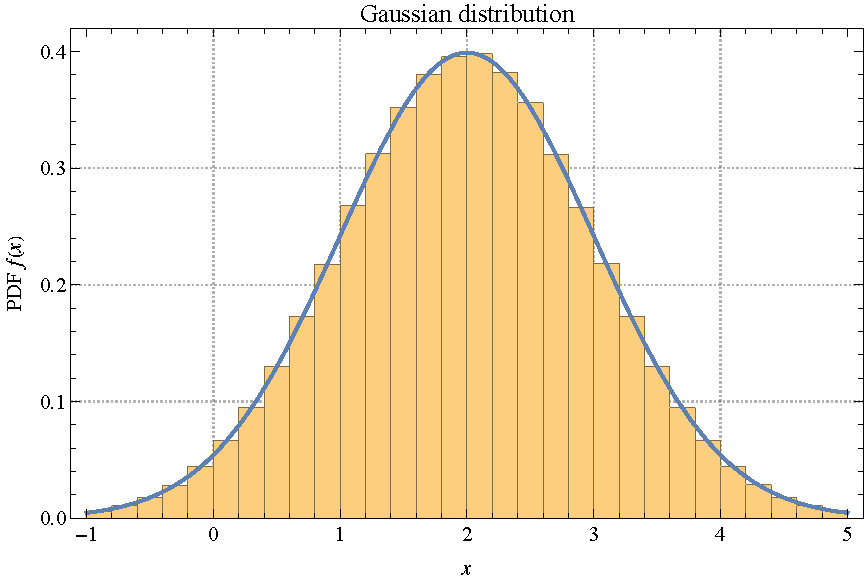
\includegraphics{exercise/change_of_var_Gaussian.pdf}
	\caption[Distribution of $x$ obeying Gaussian distribution.][6pt]{Distribution of $x$ obeying Gaussian distribution.}
	\label{fig:change_of_var_Gaussian}
\end{figure}

\begin{figure}
	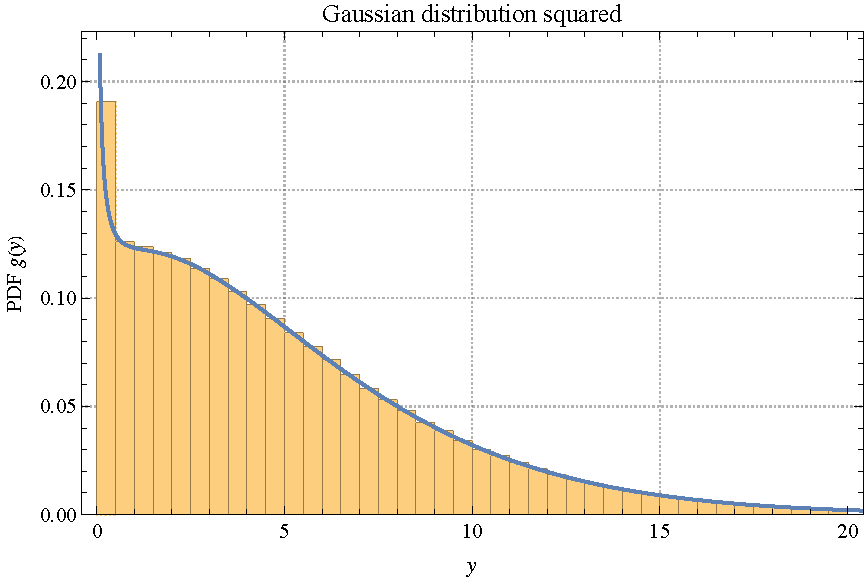
\includegraphics{exercise/change_of_var_Gaussian_squared.pdf}
	\caption[Distribution of $y = x^{2}$ from $x$ obeying Gaussian distribution.][6pt]{Distribution of $y = x^{2}$ from $x$ obeying Gaussian distribution.}
	\label{fig:change_of_var_Gaussian_squared}
\end{figure}

\paragraph{Poisson distribution}\index{Poisson distribution}

\begin{enumerate}
	\item Repeat for $x$ with a Poisson distribution with $\lambda = 3$. (Figure~\ref{fig:change_of_var_Poisson} and~\ref{fig:change_of_var_Poisson_squared})
\end{enumerate}

\begin{figure}
	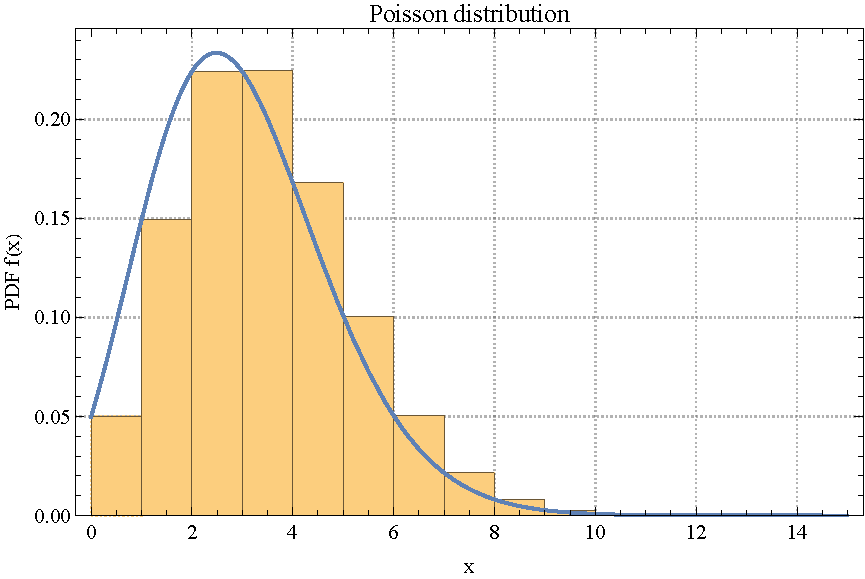
\includegraphics{exercise/change_of_var_Poisson.pdf}
	\caption[Distribution of $x$ obeying Poisson distribution.][6pt]{Distribution of $x$ obeying Poisson distribution.}
	\label{fig:change_of_var_Poisson}
\end{figure}

\begin{figure}
	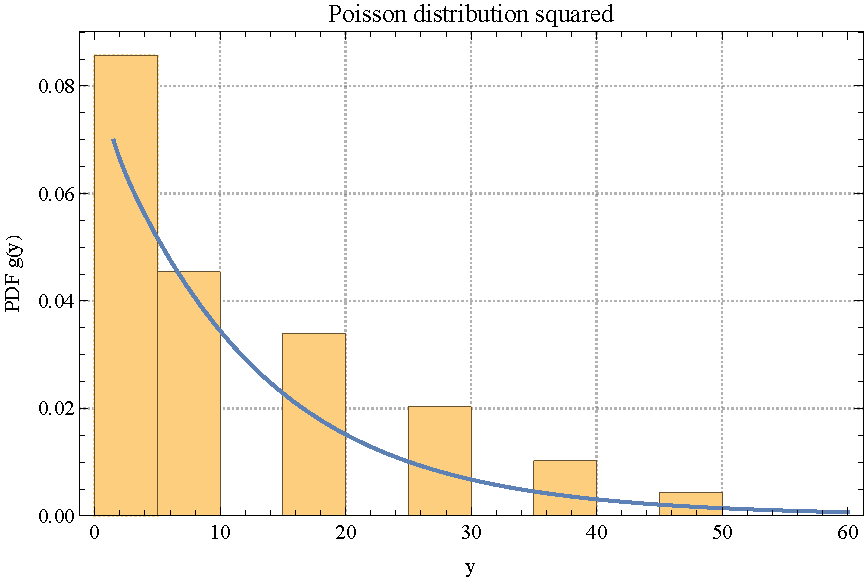
\includegraphics{exercise/change_of_var_Poisson_squared.pdf}
	\caption[Distribution of $y = x^{2}$ from $x$ obeying Poisson distribution.][6pt]{Distribution of $y = x^{2}$ from $x$ obeying Poisson distribution.}
	\label{fig:change_of_var_Poisson_squared}
\end{figure}

($\hookleftarrow$ \ref{subsec:change_of_var})

\newpage

\subsection{Ratio}\index{change of variable!ratio}
\label{exer:change_of_var_ratio}

\begin{enumerate}
	\item Take the variables $x$ and $y$, both Gaussian distributed with $\mu = 0$ and $\sigma = 1$.
	\item Compute the distribution of their ratio analytically and numerically.
\end{enumerate}

\paragraph{Analytical solution}

\begin{description}
	\item Define a change of variable: $u = \frac{x}{y}$, $v = y$.
	\item The joint-PDF\index{joint probability distribution} is:
		$$
		h(u, v) \,\mathrm{d}u \mathrm{d}v = f(x) g(y) \,\mathrm{d}x \mathrm{d}y 
		= f(uv) g(v) \left| \frac{\mathrm{d}(x, y)}{\mathrm{d}(u, v)}\right| \,\mathrm{d}u \mathrm{d}v 
		= f(uv) g(v) v \,\mathrm{d}u \mathrm{d}v
		$$
	\item The PDF\index{marginal distribution} of $u$ is:
		\marginnote[6pt]{This is the special case of Cauchy distribution\index{Cauchy distribution} with $x_{0}=0$ and $\gamma =1$, and is called the standard Cauchy distribution.}
		$$
		p(u) = \int_{-\infty}^{\infty} {f(uv)g(v)v} \,\mathrm{d}v 
		= \int_{0}^{\infty} {f(uv)g(v)v} \,\mathrm{d}v 
		= \frac{1}{\pi (1 + u^{2})}
		$$
\end{description}

\newpage

\paragraph{Numerical solution} (Figure~\ref{fig:change_of_var_ratio})

\begin{figure*}[h]
	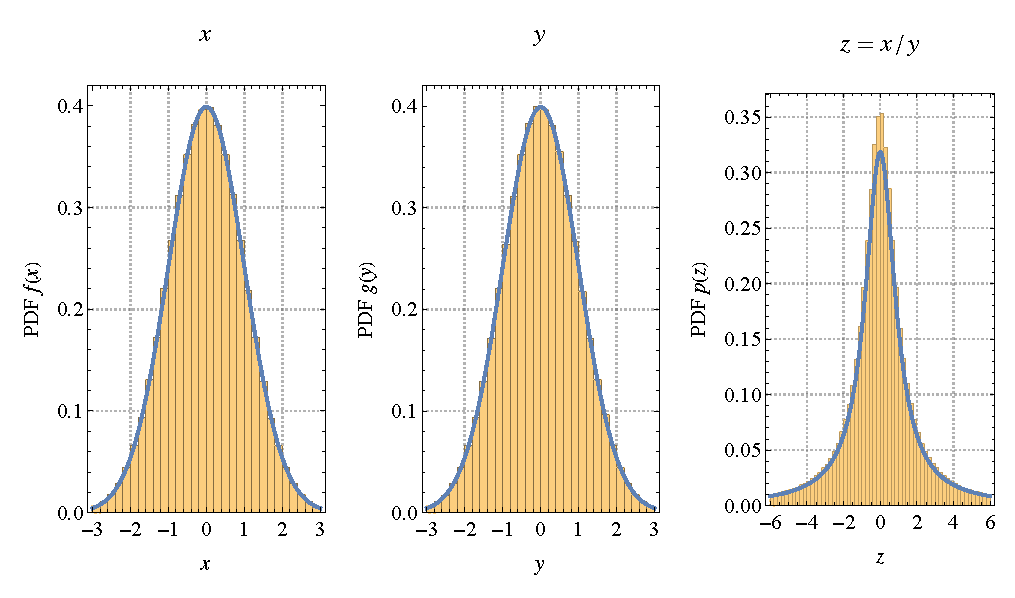
\includegraphics[width=\linewidth]{exercise/change_of_var_ratio.pdf}
	\caption[Distribution of the ratio between $x$ and $y$, both Gaussian distributed.]{Distribution of the ratio between $x$ and $y$, both Gaussian distributed with $\mu = 0$ and $\sigma = 1$.}
	\label{fig:change_of_var_ratio}
\end{figure*}

($\hookleftarrow$ \ref{subsec:prop_of_pseudorandom_number_generator})



%------------------------------------------------

\section{Binomial distribution}
\label{exer:binomial_distr}

\subsection{Generate binomial variables}

\begin{enumerate}
		\marginnote{Do not use any predefined method for the binomial or factorial.}
	\item Compute the distribution of binomial variables $k_{i}$ with $n = 150$ and $pi = \{ 0.1, 0.3, 0.5, 0.7, 0.9 \}$.
	\item Plot them all together.
	\item Repeat for $n = 500$.
\end{enumerate}

\subsection{Hints for the solution}

Compute the binomial coefficient using $a = \exp( \ln(a) )$, and simplify the terms that cancel out:

\begin{equation}
	\mathrm{BinomialCoeff}(n, k) 
	= \exp \left[ \sum_{i = n - k + 1}^{n}{\ln(i)} - \sum_{i = 2}^{k}{\ln(i)} \right]
\end{equation}

Compute the Bernoulli term with $a = \exp( \ln(a) )$ to avoid numerical problems in the situation that $p$ is small and $(1 - p)$ large, or viceversa:

\begin{equation}
	p^{k}(1 - p)^{n - k} = \exp \left[ k \ln(p) + (n - k) \ln(1 - p) \right]
\end{equation}

(Figure~\ref{fig:binomial_distr_n_150} and~\ref{fig:binomial_distr_n_500})

\begin{figure}
	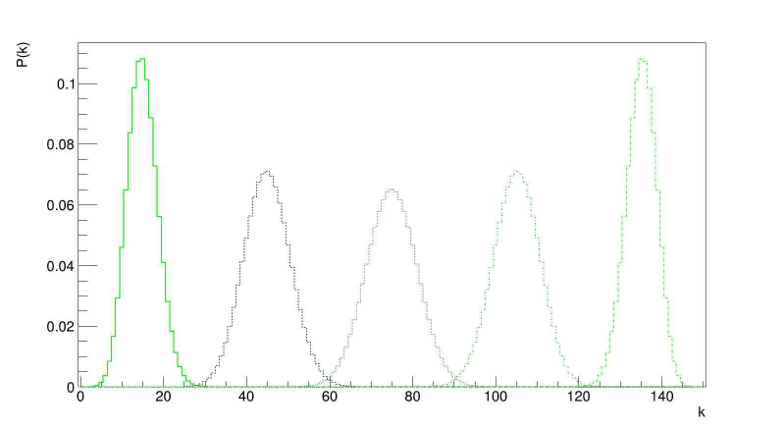
\includegraphics{exercise/binomial_distr_n_150.png}
	\caption[Binomial distribution ($n = 150$).][6pt]{Binomial distribution ($n = 150$).}
	\label{fig:binomial_distr_n_150}
\end{figure}

\begin{figure}
	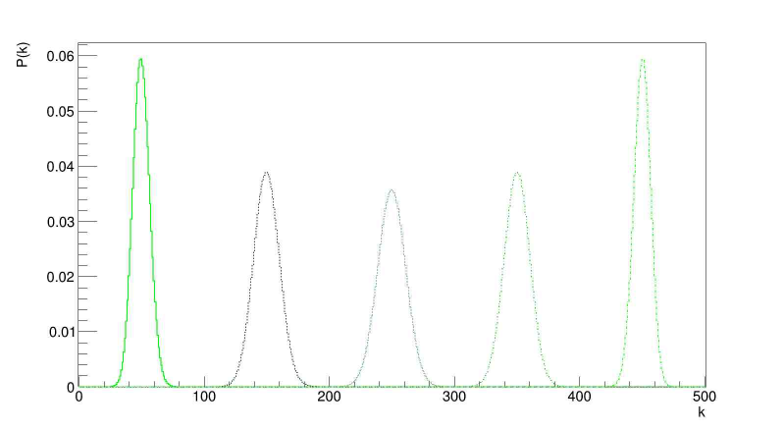
\includegraphics{exercise/binomial_distr_n_500.png}
	\caption[Binomial distribution ($n = 500$).][6pt]{Binomial distribution ($n = 500$).}
	\label{fig:binomial_distr_n_500}
\end{figure}

($\hookleftarrow$ \ref{subsec:binomial_distr})



%------------------------------------------------

\section{Exponential from uniform}
\label{exer:expo_from_uniform}

\subsection{Generate exponential variables from uniform}

\begin{enumerate}
	\item Generate $10^{6}$ values of the variable $t$, uniformly distributed in $[0, \Delta t = 10^{3}]$.
	\item Sort the list of generated values.
	\item Compute the interval $\delta t_{i} = t_{i} - t_{i - 1}$.
	\item Plot the distribution of $\delta t_{i}$ (as a histogram).
	\item Fit it with an exponential. 
		\marginnote{Does it work? Do you get back the input parameters?}
\end{enumerate}

\subsection{Hints for the solution}

Fit the histogram with the following function:

\begin{equation}
	f(\delta t) = n \cdot \lambda_{1} \cdot w_{t} \cdot \mathrm{e}^{- \lambda_{2} \cdot \delta t}
\end{equation}

where: $n = 10^{6}$ (fixed value) and $w_{t} = $ bin width (fixed).

At this point, we need to make sure that the fit outputs the same values for $\lambda_{1}$ and $\lambda_{2}$.

Alternatively, we can fit with:

\begin{equation}
	f(\delta t) = n \cdot \lambda \cdot w_{t} \cdot \mathrm{e}^{- \lambda \cdot \delta t}
\end{equation}

but leaving $n$ a free parameter.

In this case, the fit should return $n = 10^{6}$.

(Figure~\ref{fig:expo_from_uniform})

\begin{figure}
	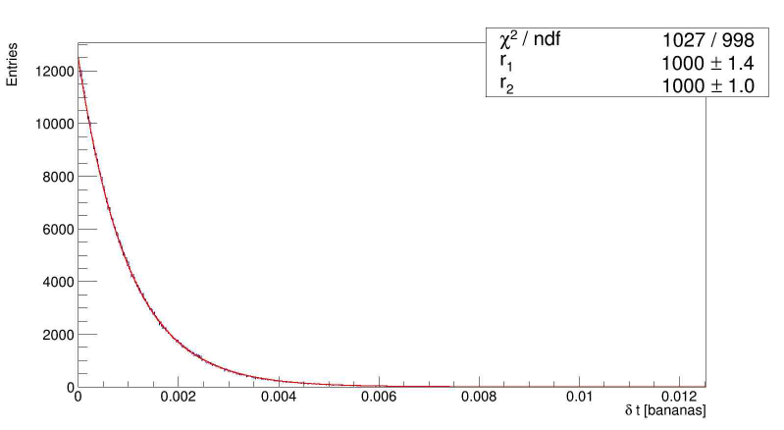
\includegraphics{exercise/expo_from_uniform.png}
	\caption[Exponential from uniform.][6pt]{Exponential from uniform.}
	\label{fig:expo_from_uniform}
\end{figure}

($\hookleftarrow$ \ref{subsec:expo_distr})



%------------------------------------------------

\section{Poisson distribution}
\label{exer:poisson_distr}

\subsection{Generate Poisson variables}

\begin{enumerate}
		\marginnote{Do not use any predefined method for the binomial and Poisson distribution.}
	\item Generate $n = 10$ uniformly distributed values of $t$ in $[0, \Delta t = 10^{3}]$.
	\item Compute the number of accepted events $k$ that happen in interval $[0, \delta t]$, with $\delta t = p \cdot \Delta t$ t and $p = 0.01$.
	\item Repeat $10^{5}$ times, and populate the histogram of $k$.
	\item Plot the histogram of $k$ and compare it with the theoretical binomial and Poisson distribution.
	\item Repeat for all combinations of: $n = \{ 10, 100, 1000 \}$ and $p = \{ 0.01, 0.05, 0.1, 0.5 \}$.
\end{enumerate}

(Figure~\ref{fig:Poisson_distr})

\begin{figure}
	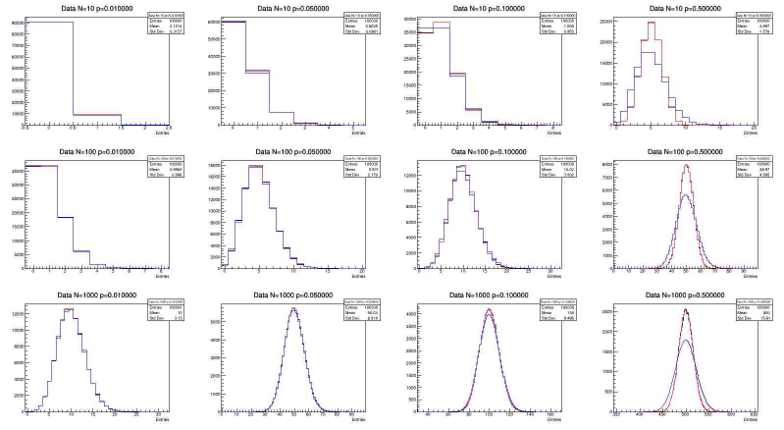
\includegraphics{exercise/Poisson_distr.png}
	\caption[Poisson distribution.][6pt]{Poisson distribution.}
	\label{fig:Poisson_distr}
\end{figure}

($\hookleftarrow$ \ref{subsec:poisson_distr})



%------------------------------------------------

\section{Sum of normally distributed random variables}
\label{exer:sum_of_Gaussian}

\subsection{Normally distributed and uncorrelated does not imply independent}

Two normally distributed, uncorrelated but dependent variables.

Suppose $X$ has a normal distribution with expected value 0 and variance 1. Let $W$ have the Rademacher distribution, so that 

\begin{equation}\label{eq:Rademacher_distr}
	w(x) = \left\{
	\begin{array}{ccl}
		\frac{1}{2} & & {\textrm{if } W = 1}\\
		\frac{1}{2} & & {\textrm{if } W = - 1}\\
		0 & & {\textrm{otherwise}}
	\end{array} \right.
\end{equation}

and assume $W$ is independent of $X$. Let $Y=WX$. Then
\begin{itemize}
	\item $X$ and $Y$ are uncorrelated;
	\item both have the same normal distribution;
	\item and $X$ and $Y$ are not independent.
\end{itemize}

The joint probability distribution is shown in Figure~\ref{fig:joint_pdf_sum_of_Gaussian}.

\begin{figure}
	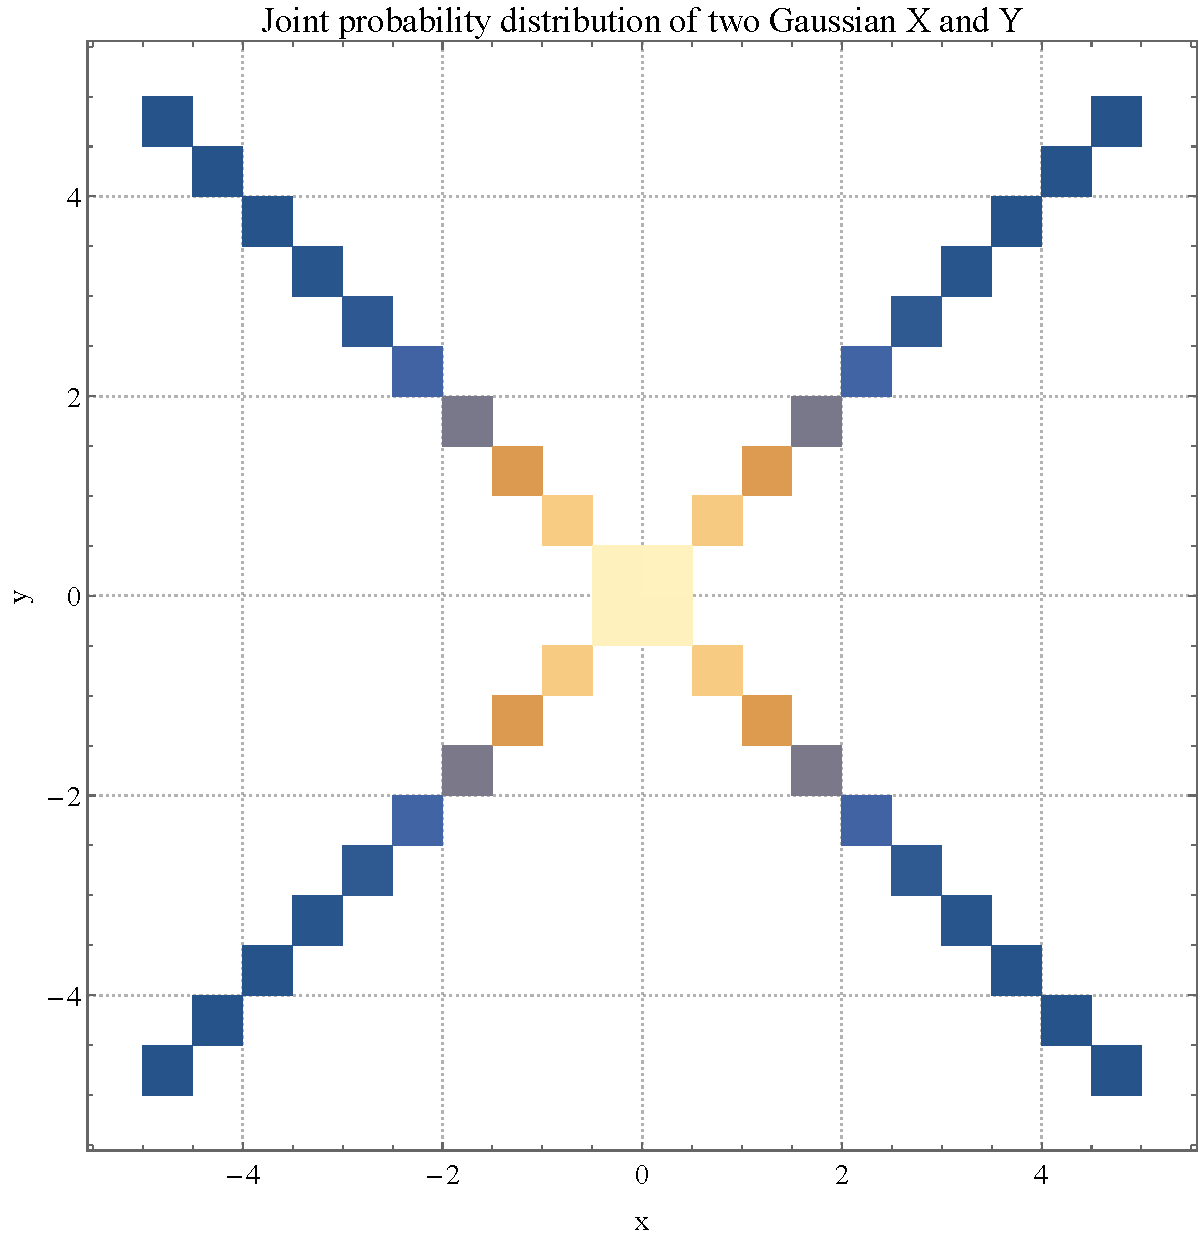
\includegraphics{exercise/joint_pdf_of_two_Gaussian.pdf}
	\caption[Joint probability distribution of two “normal” variables $X$ and $Y$.][6pt]{Joint probability distribution of two “normal” variables $X$ and $Y$.}
	\label{fig:joint_pdf_sum_of_Gaussian}
\end{figure}

To see that $X$ and $Y$ are uncorrelated, one may consider the covariance $\mathrm{cov} (X,Y)$: by definition, it is

$$
\mathrm{cov}(X, Y) = \mathrm{E}(XY) - \mathrm{E}(X) \mathrm{E}(Y)
$$

Then by definition of the random variables $X$, $Y$, and $W$, and the independence of $W$ from $X$, one has

$$
\mathrm{cov}(X, Y)= \mathrm{E}(XY) - 0 = \mathrm{E}(X^{2} W) = \mathrm{E}(X^{2}) \mathrm{E}(W) = \mathrm{E}(X^{2}) \cdot 0 = 0
$$

To see that $Y$ has the same normal distribution as $X$, consider

$$
\begin{array}{rl}
	P(Y \leq x) &= \mathrm{E}(P(Y \leq x \mid W))\\
	&= P(X \leq x) P(W = 1) + P(- X \leq x) P(W = -1)\\
	&= \Phi(x) \cdot \frac{1}{2} + \Phi(x) \cdot \frac{1}{2}
\end{array}
$$

\marginnote{Since $X$ and $- X$ both have the same normal distribution.}

where $\Phi(x)$ is the cumulative distribution function of the standard normal distribution.

To see that $X$ and $Y$ are not independent, observe that

$$
P(Y > 1 \mid - \frac{1}{2} < X < \frac{1}{2}) = P( X > 1 | - \frac{1}{2} < X < \frac{1}{2}) = 0
$$

Finally, the distribution of the simple linear combination $X + Y$ concentrates positive probability at 0 (Figure~\ref{fig:sum_of_Gaussian}): 

$$
P(X + Y = 0) = \frac{1}{2}
$$

Therefore, the random variable $X + Y$ is not normally distributed, and so also $X$ and $Y$ are not jointly normally distributed. 

\begin{figure}
	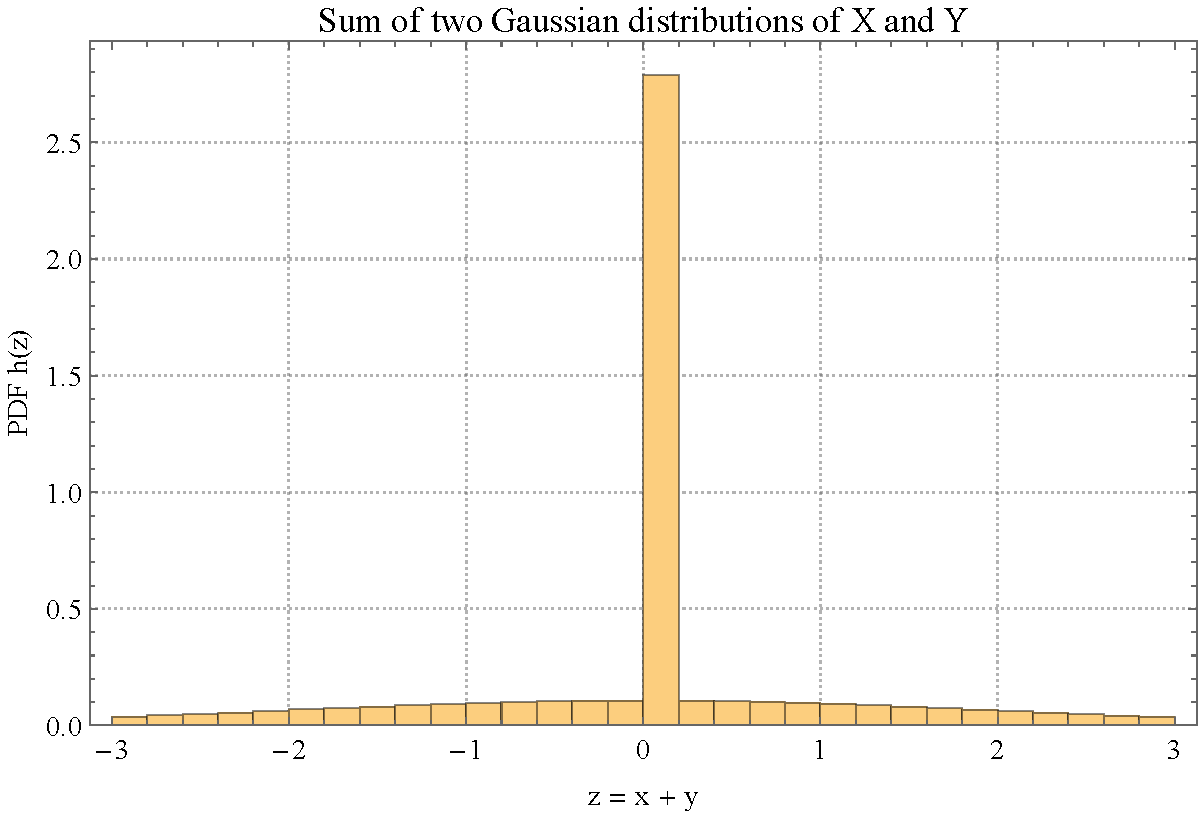
\includegraphics{exercise/sum_of_Gaussian.pdf}
	\caption[Probability distribution of the sum of two “normal” variables.][6pt]{Probability distribution of the sum of two “normal” variables $X$ and $Y$.}
	\label{fig:sum_of_Gaussian}
\end{figure}

($\hookleftarrow$ \ref{subsec:prop_of_gaussian_distr})



%------------------------------------------------

\newpage

\section{$\chi^{2}$ distribution}
\label{exer:chisquare_distr}

\subsection{Generate $\chi^{2}$ distribution}

\begin{enumerate}
	\item Generate $10^{5}$ sets of $n$ standard normal variables $\chi$, and populate the histogram with $X^{2} = \sum_{i = 1}^{n}{\chi^{2}}$.
	\item Repeat 1. for $n = \{ 1, 2, 3, 5, 10, 20 \}$.
	\item Plot the histograms and overlap them with the theoretical $\chi^{2}$ distribution with the corresponding number of degrees of freedom, properly scaled to the number of generated values.
\end{enumerate}

(Figure~\ref{fig:chisquare_distr})

\begin{figure}
	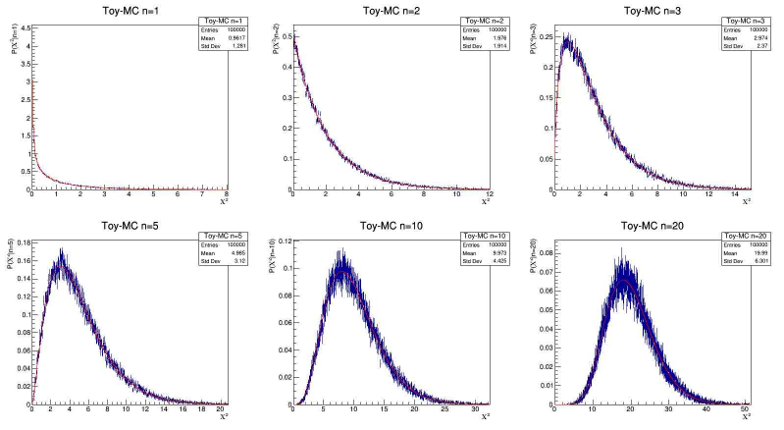
\includegraphics{exercise/chisquare_distr.png}
	\caption[$\chi^{2}$ distribution.][6pt]{$\chi^{2}$ distribution.}
	\label{fig:chisquare_distr}
\end{figure}

($\hookleftarrow$ \ref{subsec:chisquare_distr})



%------------------------------------------------

\newpage

\section{Gaussian random number generator}
\label{exer:gaussian_random_number_generator}

\subsection{Central limit for Gaussian random number generator}

\begin{enumerate}
	\item Generate $10^{8}$ sets of $n$ uniformly distributed random variables in $[0, 1)$, with $n = \{ 1, 2, \cdots,10 \}$.
	\item For every $n$, populate a histogram with the $10^{8}$ sums of the $n$ generated random numbers.
	\item Plot the histogram in linear and log-scale. 
		\marginnote{Do you notice anything?
		
		One can demonstrate that the distribution will be cut off at $\pm \sqrt{3n}$.}
\end{enumerate}

(Figure~\ref{fig:gaussian_random_number_generator} and~\ref{fig:gaussian_random_number_generator_logy})

\begin{figure}
	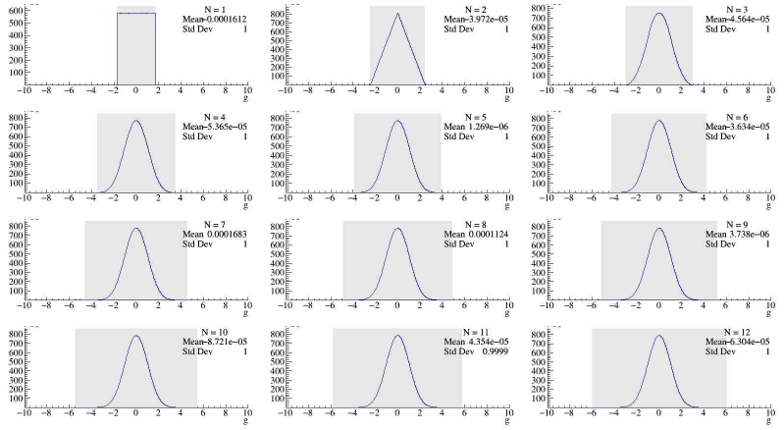
\includegraphics{exercise/gaussian_random_number_generator.png}
	\caption[Central limit for Gaussian random number generator.][6pt]{Central limit for Gaussian random number generator.}
	\label{fig:gaussian_random_number_generator}
\end{figure}

\begin{figure}
	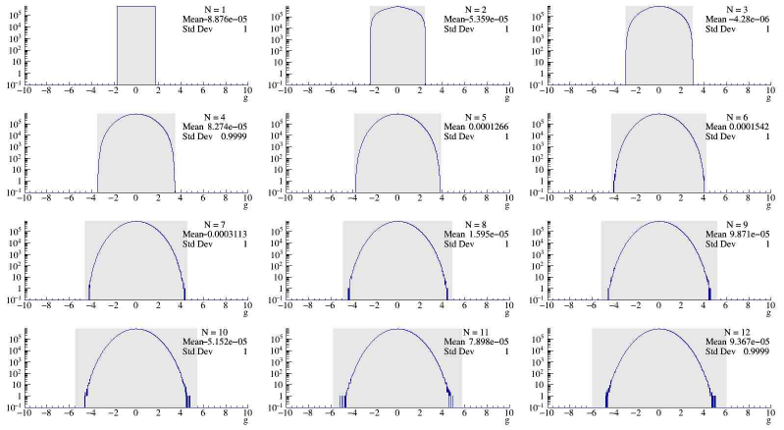
\includegraphics{exercise/gaussian_random_number_generator_logy.png}
	\caption[Central limit for Gaussian random number generator with log-scale.][6pt]{Central limit for Gaussian random number generator with log-scale.}
	\label{fig:gaussian_random_number_generator_logy}
\end{figure}

($\hookleftarrow$ \ref{subsec:central_limit_theorem})



%------------------------------------------------

\section{Acceptance-Rejection method}
\label{exer:acceptance_rejection}

\subsection{Hit-or-miss method}

\begin{enumerate}
	\item Generate $10^{6}$ points uniformly distributed with $x \in [-1, 1]$ and $y \in [-1, 1]$.
	\item Compute the fraction of points falling inside a circle of radius 1.
	\item Repeat for $\mathrm{dim} = \{ 2, 3, 4, \cdots, 15 \}$.
	\item Plot the fraction of accepted points as a function of the dimension.
	\item Assign an uncertainty to your estimate of accepted points.
	\item Compare the plot with the theoretical expectation.
\end{enumerate}

\subsection{Hints for the solution}

The theoretical expectation is the ratio between the volume of an n-dimensional sphere and $2^{n}$.

As an uncertainty, we can use the variance of the binomial distribution.

(Figure~\ref{fig:acceptance_rejection})

\begin{figure}
	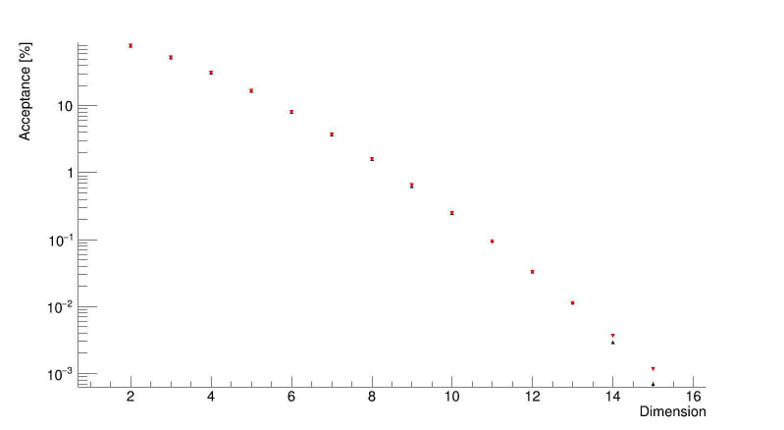
\includegraphics{exercise/acceptance_rejection_method.png}
	\caption[Acceptance as a function of the dimension.][6pt]{Acceptance as a function of the dimension for acceptance rejection method.}
	\label{fig:acceptance_rejection}
\end{figure}

($\hookleftarrow$ \ref{subsec:acceptance_rejection})



%------------------------------------------------

\newpage

\section{Random number correlation}
\label{exer:random_number_corr}

\subsection{Random number correlation in Metropolis–Hastings algorithm}

\begin{enumerate}
	\item Generate $10^{5} + 1$ random numbers distributed as a Gaussian with $\mu = 3$ and $\sigma = 2$.
	\item Plot the distributions of $x_{i}$ and of $\delta x_{i} = (x_{i} - x_{i - 1})$.
	\item Repeat by generating the numbers $x_{i}$ with the Metropolis-Hastings algorithm until $10^{5} + 1$ points are accepted.
	\item As a proposal function, use a Gaussian with $\mu_{p} = x_{i}$ and $\sigma = 0.3$.
	\item How do the distributions look like?
	\item Can you explain the standard deviation of the $\delta x_{i}$ distribution in the two cases?
\end{enumerate}

(Figure~\ref{fig:random_number_corr})

\begin{figure}
	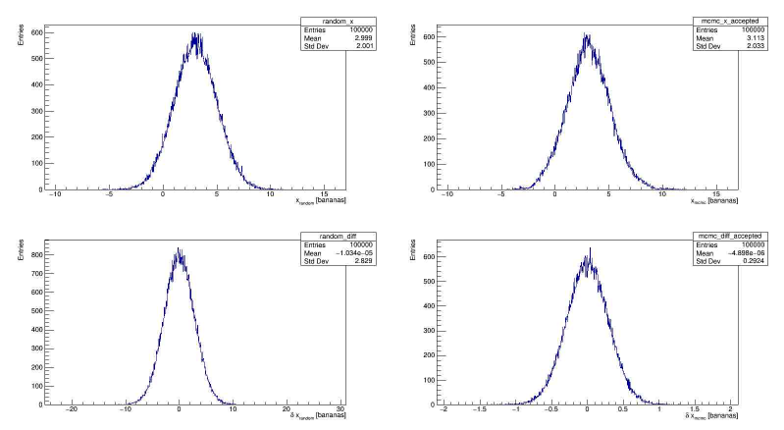
\includegraphics{exercise/random_number_corr.png}
	\caption[Random number correlation in Metropolis–Hastings algorithm.][6pt]{Random number correlation in Metropolis–Hastings algorithm.}
	\label{fig:random_number_corr}
\end{figure}

($\hookleftarrow$ \ref{subsec:prop_of_metropolis})



%----------------------------------------------------------------------------------------

\backmatter

%----------------------------------------------------------------------------------------
%	BIBLIOGRAPHY
%----------------------------------------------------------------------------------------

\bibliography{bibliography} % Use the bibliography.bib file for the bibliography
\bibliographystyle{plainnat} % Use the plainnat style of referencing

%----------------------------------------------------------------------------------------

\printindex % Print the index at the very end of the document

\end{document}
